%%%%%%%%%%%%%%%%%%%%%%%%%%%%%%%%%%%%%%%%%%%%%%%%%%%%%%%%%%%%%%%%%%%%%%%
%                 UNIVERSIDAD NACIONAL DE INGENIAR�A                  %
%           Facultad de Ingenier�a Industrial y de Sistemas           %
%                                                                     %
%                  | FORMATO DE PROPUESTA DE TESIS |                  %
%                                                                     %
%                     (C) Samuel Oporto D�az                          %
%                         soporto@wiphala.net                         %
%                         Carlos Mauro C�rdenas Fern�ndez             %
%                         unimauro@gmail.com                          %
%                                                                     %
%                              Lima - 2007                            %
%%%%%%%%%%%%%%%%%%%%%%%%%%%%%%%%%%%%%%%%%%%%%%%%%%%%%%%%%%%%%%%%%%%%%%%

% -------------------------------------------------
% define par�metros del d0000000000000000000000000000000000ocumento
% -------------------------------------------------
\documentclass[12pt,a4paper]{report}


\usepackage{0.proposal_uni_fiis}
%\usepackage{amsmath}
\usepackage[latin1]{inputenc}

%\usepackage[ascii]{inputenc}
\usepackage[T1]{fontenc}
\usepackage[scaled]{uarial}
\renewcommand*\familydefault{\sfdefault}
\usepackage[spanish]{babel}
\usepackage{amsmath,amssymb,amsfonts,textcomp}
\usepackage{ifpdf}
%\usepackage{uarial}
\usepackage{setspace}
\usepackage{color}
\usepackage{array}
\usepackage{hhline}
%\usepackage{hyperref}
\usepackage{textcomp}
\usepackage{times}
\usepackage{datetime}
\usepackage{titlesec}
\usepackage{placeins}
\usepackage{subfigure}
\usepackage{supertabular}
\usepackage{longtable}
\usepackage{colortbl}
\usepackage{lscape}
\usepackage{fullpage,graphicx}
\usepackage[pdftex]{hyperref}
\usepackage[nottoc]{tocbibind} 
\usepackage{rotating}
\usepackage{multirow}
\usepackage{inputenc}
\usepackage{sectsty}
\sectionfont{\normalsize\MakeUppercase}
\subsectionfont{\normalsize\MakeUppercase}
\subsubsectionfont{\normalsize\MakeUppercase}
\usepackage[left=4cm,top=4cm,right=2.5cm,bottom=2.5cm]{geometry} 
%AGREGAR AQUI MAS PAQUETES
% -------------------------------------------------
% define datos del tesista
% -------------------------------------------------
\uniauthorA{Carlos Mauro C�rdenas Fern�ndez}              %% Autor de la propuesta
%\unicodeA{19990039F}                                      %% C�digo Alumno
%\uniauthorB{Palermo Ston, Pedro Adelante}                %% Autor de la propuesta
%\unicodeB{2000003C}                                      %% C�digo Alumno

%\unimonth{31 de Julio}                                     %% Mes de propuesta
\uniyear{2009}                                           %% A~no de propuesta
%\unicycle{2009-I}                                       %% Periodo acad�mico
\unicity{Lima Per�}                                    %% Ciudad

%\unititle{Usabilidad de Software Sugar de las OLPC}
\unititle{EVALUACI�N DE LA OLPC CON INGENIER�A DE USABILIDAD}
\engtitle{EVALUATING THE OLPC WITH USABILITY ENGINEERING}
                                                         %% Titulo de la prop.
%\unimajor{Ing.~Arturo Simich}                    %% Asesor de propuesta.
%\engmajor{Arturo Simich, Eng}                    %% Major Professor
%\unidirector{Ing.~Gloria Teresita Huamani}                   %% Director de Escuela

\uniuni{UNIVERSIDAD NACIONAL DE INGENIER�A}              %% Universidad
\unifac{FACULTAD DE INGENIER�A INDUSTRIAL Y DE SISTEMAS} %% Facultad
\engfac{FACULTY OF INDUSTRIAL ENGINEERING AND SYSTEMS}   %% Faculty
%\engfac{Faculty of Industrial Engineering and Systems}   %% Faculty
%\uniesc{Escuela Profesional de Ingenier�a de Sistemas}   %% Escuela
\unigrade{INGENIER�A DE SISTEMAS}                         %% Nombre del grado academico.
% -------------------------------------------------
% silabeo
% -------------------------------------------------
\hyphenation {
a-na-li-zan
a-nor-ma-li-dad
a-rra-ci-ma-dos
a-rre-glo
a-so-cia-das
va-lor
ma-yor
}

%----------------

%----------------


%----------------
%%%%%%%%%%%%%%%%%%%%%%%%%%%%%%%%%%%%%%%%%%%%%%%%%%%%%%%%%%%%%%%%%%%%%%%%%%%%%%%%%%%%%%%%%%%%%%
%% Formato que le solicitaron a Jonhatan Zelada usada por BENITO ZARATE
%%%%%%%%%%%%%%%%%%%%%%%%%%%%%%%%%%%%%%%%%%%%%%%%%%%%%%%%%%%%%%%%%%%%%%%%%%%%%%%%%%%%%%%%%%%%%%
%%%\titleformat{\chapter}[display]
%%%\renewcomand{\thechapter}{\thechapter : }
%%%\renewcomand{\thechapter}{\Roman{chapter}:}
%%\titleformat{\chapter}[hang]
%%%{\vspace*{2cm}}
%%%{\vspace{20ex}
%%{\centering\vspace*{2cm}\large\bfseries}
%%%{\filcenter
%%%{\vspace{8cm}}
%%\MakeUppercase{\MakeUppercase{\chaptertitlename}\enspace \large\MakeUppercase{\thechapter} :}{\large\MakeUppercase}
%%{\vspace{1ex}}{\vspace{1ex}}
%%%\filcenter}
%----------------
%%%%%%%%%%%%%%%%%%%%%%%%%%%%%%%%%%%%%%%%%%%%%%%%%%%%%%%%%%%%%%%%%%%%%%%%%%%%%%%%%%%%%%%%%%%%%%

%-------------------------------------------------------------------------------------------
%%%%%%%%%%%%%%%%%%%%%%%%%%%%%%%%%%%%%%%%%%%%%%%%%%%%%%%%%%%%%%%%%%%%%%%%%%%%%%%%%%%%%%%%%%%%%%
%% 
%%	Formalo exigido por Ciriano que joda...
%%
%%%%%%%%%%%%%%%%%%%%%%%%%%%%%%%%%%%%%%%%%%%%%%%%%%%%%%%%%%%%%%%%%%%%%%%%%%%%%%%%%%%%%%%%%%%%%%
\titleformat{\chapter}[display]
  {\normalfont\MakeUppercase\large\bfseries\centering\vspace*{2cm}}{\large\MakeUppercase{\chaptertitlename}\ \large\MakeUppercase{\large\thechapter}}{14pt}{\large\MakeUppercase}
%-------------------------------------------------------------------------------------------


%----------------
\titleformat{\tableofcontents}[display] % cambiamos el formato de los cap�tulos
{\bfseries\huge} % por defecto se usar�n caracteres de tama�o \Huge en negrita
{% contenido de la etiqueta
% \titlerule % l�nea horizontal
 \vspace*{1.8cm}
 %\vskip2.5cm 
 \filcenter % texto alineado a la derecha
 \huge\contentsname\ % "Cap�tulo" o "Ap�ndice" en tama�o \Large en lugar de \Huge
 %\huge\thechapter} % n�mero de cap�tulo en tama�o \Large
{5mm} % espacio m�nimo entre etiqueta y cuerpo
{\filcenter} % texto del cuerpo alineado a la derecha
%[\vspace{0.5mm} \bigrule]



% -----------------------
\begin{document}
\onehalfspacing
\bibliographystyle{alpha}

\unibuildpaste        % pasta de la propuesta
\unibuildcover        % car�tula de la propuesta
\newpage
\uniacknowledgment    % reconocimientos
\newpage
\uniackprolog
\newpage
\uniabstractspa       % resumen en espa�ol
\uniabstracteng       % resumen en ingl�s

\frontmatter


\newpage
\setcounter{page}{1}
\pagenumbering{roman} 

\tableofcontents
\listoftables
\listoffigures
\descriptores

\newpage
\mainmatter 
\setcounter{page}{1}  
\pagenumbering{arabic} 
%\chapter{Introducci�n}
%\chapter{INTRODUCCI�N}
%\chapter{Introducci�n}
%\vspace*{8cm}
%\vskip3cm 
\chapter*{\vskip1cm Introducci�n}
\addcontentsline{toc}{chapter}{Introducci�n}
\label{chapter.Introduccion}
% ----------------------------------------------
%\linespread{1.3}

\begin{figure}[ht]
	\centering
		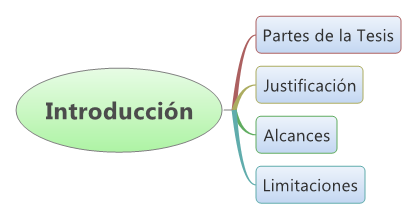
\includegraphics{./img/MapaMental/capitulo01.png}
	\caption{Mapa Mental del Cap�tulo de Introducci�n}
	\label{Mapa Mental del Capitulo de Introduccion}
\end{figure}


%\section*{Introducci�n}
%\addcontentsline{toc}{section}{Introducci�n}
%\label{section.Introduccion}

Se est� llevando un proceso de singularidad tecnol�gica en todos los aspectos de la vida del ser humano dentro del trabajo, salud, transporte, comunicaci�n y la educaci�n. Es com�n en pa�ses desarrollados, del norte, el uso de las tecnolog�as de informaci�n y comunicaciones (TICs) por medio de los tel�fonos, internet, computadoras de escritorio o laptops transversalmente a las actividades productivas agregando mas valor a sus productos finales. Esta realidad no se traslada totalmente a la poblaci�n en otros paises ubicados al sur, encontr�ndose barreras de entradas fundamentalmente econ�micas y de acceso a la tecnolog�a\footnote{El Estudio Sobre la Audiencia de Internet publicado por Comscore el 23 de enero del 2009 rebela que los paises que conforman el G8(Estados Unidos, Gran Breta�a, Italia, Francia, Alemania, Jap�n, Canad� y Rusia) tienen el 40\% del total de los internautas a nivel mundial. Seg�n el estudio sobre \textbf{La Distribuci�n Mundial de la Riqueza de los Hogares} por el Instituto Mundial para la Investigaci�n de Desarrollo Econ�mico de la Universidad de las Naciones Unidas. El 88\% de la riqueza el mundo est� en Estados Unidos, Europa y Paises de Asia Pac�fico Ricos. 

Fuente: http://www.comscore.com/press/release.asp?press=2698 . 

http://www.wider.unu.edu 16/02/2009}. En el campo de la educaci�n la incursi�n de las TICs en las aulas se aceler� de forma heterog�nea, increment�ndose de brecha digital en los centros urbano de instituciones privadas a los centros educativos rurales o urbano marginales\footnote{Seg�n el Informe T�nico del Instituto Nacional de Estad�stica e Inform�tica INEI: Tecnolog�as de la Informaci�n y  Comunicaci�n en los Hogares en junio del 2008 las zonas rurales poseen una muy baja participaci�n en las TICs .\cite{inforinei}}. Los gobiernos intentan incrementar las pol�ticas de inclusi�n digital en �reas elementales de la educaci�n, pero a�n se tiene muchos limitantes por el aspecto geogr�fico y financiero\footnote{ El Acuerdo Nacional del Per� del a�o 2002 establece garantizar�recursos para la reforma educativa otorgando un incremento m�nimo anual en el presupuesto del sectoreducaci�n equivalente al 0.25 \% del PBI, hasta que �ste alcance un monto global equivalente a 6\% del PBI. \cite{AN2002}. El presupuesto p�blico para educaci�n del 2009 es menor al 3\% del PBI seg�n el Sindicato Unico de Trabajadores de la Educaci�n del Per� SUTEP. 

Fuente: http://www.ipp-peru.com/upload/PRESUPUESTO\_EDUCACION\_2009\_dic.pdf 16/02/2009  }. 

Sin embargo la incursi�n de las TICs est� en aumento las aulas gracias a cinco factores. El primero con iniciativas privadas, de gobierno y civiles; apoyadas inclusive por organismos internacionales como la Organizaci�n de Naciones Unidas, este �ltimo por medio del Fondo de Naciones Unidas para la Infancia UNICEF. El segundo factor es la disminuci�n de costos del hardware, su continuo desarrollo de nuevos equipos con precios en constante descenso debido a la reducci�n del ciclo de vida de sus productos\footnote{La Ley de Moore expresa que aproximadamente cada 18 meses duplica el n�mero de transistores en un circuito integrado. Fuente: http://es.wikipedia.org/wiki/Ley\_de\_Moore 16/02/2009 }. El tercer factor es el software y en particular el software libre\footnote{Libertades del Software Libre: 0.Uso, 1.Compartir, 2.Modificar y 3.Distribuir. 

Fuente: www.gnu.org/philosophy/free-sw.es.html 16/02/2009 } impulsado por una comunidad mundial distribuida, y cada vez mas profesionales ocupados en software educativo para el proceso de ense�anza, aprendizaje y control generando muchas espectativas en la comunidad educativa\footnote{En el portal de proyecto de SourceForge(www.sf.net) se tienen 10704 proyectos sucritos 16/02/2009.}. El cuarto factor es la conectividad que brinda la internet con potencial para acceder al conocimiento y con ello mejorar los niveles de ingreso y de vida de la poblaci�n a futuro. El quinto factor es el educativo, nuevas investigaciones y propuestas para enfrentar los nuevos paradigmas del incremento de la complejidad, inclusi�n de las herramientas TICs y del conocimiento con tendencia al dominio p�blico a disposici�n del maestro, padre de familia y alumno ubicando nuevos roles dentro del aula. Visionarios como Seymour Papert (1980)\cite{01SeyPapert1980} han defendido siempre el uso de la tecnolog�a inform�tica como un instrumento de apoyo a los ni�os en el aprendizaje autodirigido.

Amparados en estos cinco factores se soportan iniciativas internacionales como el proyecto de Una Laptop por Ni�o de siglas OLPC en ingl�s del cual la presente tesis se encargar� de hacer una evaluaci�n de usabilidad del software SUGAR en ni�os que la usen por primera vez para conseguir la informaci�n: "Si la experiencia de los ni�os en ellas genera aceptaci�n y comodidad en su uso".

La tesis es motivada por la curiosidad de conocer la adaptaci�n de los ni�os al usar las OLPC con SUGAR. Se recolect� datos cualitativos y cuantitativos. Se explayar� en conceptos fundamentales del �rea de Interacci�n Humano Computador IHC o Human Computer Interaction HCI en ingles, en especial de la Ingenier�a de Usabilidad. El estudio de campo y colecci�n de datos con test de usabilidad en ni�os de 5 a 7 a�os de un colegio Urbano Marginal de Lima, Per�. El instrumento para recoger la informaci�n son las pruebas de usabilidad. Los resultados ayudan a  tener mejores apreciaciones sobre el impacto del uso del software SUGAR de las OLPC, as� como medir la usabilidad, despejando las hip�tesis referedidas sobre el beneficio de usar Sugar en las OLPC.

\section*{Partes de la Tesis}
\addcontentsline{toc}{section}{Partes de la Tesis}
\label{section.partesdelatesis}

La Tesis estar� dividida de la manera siguiente:

En la \textbf{Introducci�n} se tratar� acerca de la justificaci�n y definici�n de los alcances y limitaciones de la propuesta de tesis. En el \textbf{cap�tulo \ref {chapter.Formulacion.del.Problema} Formulaci�n del Problema} se describir� de la situaci�n problem�tica con las OLPC y su software, descripci�n del problema, el objetivo de la investigaci�n y los �rboles de problemas y objetivos. En l \textbf{cap�tulo \ref {chapter.Marco.Teorico} Marco Te�rico} con tres secciones: Proyecto Una Laptop Por Ni�o describe el proyecto. En la Software y Aprendizaje se explicar� la importacia del uso del software con los ni�os. En la secci�n Ingenier�a de Usabilidad se detallar�n conceptos acerca de sus t�cnicas, m�todos y antedecentes de estudios de la usabilidad en la OLPC. En el \textbf{cap�tulo \ref{Metodologia.de.la.Investigacion}  Investigaci�n} se tratar� sobre el tipo de investigaci�n usado en la tesis. En la secci�n Dise�o de la Investigaci�n se tratar� el objeto de la investigaci�n, dise�o de la investigaci�n, dise�o de la investigaci�n y la hip�tesis.  En la secci�n Gestion de la Investigaci�n se tratar� descripci�n de la gesti�n del proyecto de tesis, actividades, recursos necesarios, cronograma de trabajo y presupuesto de la investigaci�n en un intento de usar la metolog�a pmi. En el \textbf{cap�tulo \ref{chapter.Modelo.de.Solucion} Modelo de Soluci�n} se tratar� el modelo de soluci�n, muestreo primario, recolecci�n de datos cuantitativos, dise�o del test, ejecuci�n del test piloto, an�lisis de resultados y la redacci�n de la tesis. En el \textbf{cap�tulo \ref {chapter.Analisis.de.Resultados} An�lisis de Resultados} se tratar� la operacionalizaci�n de las variables, instrumentos de medici�n y el muestreo. En el \textbf{cap�tulo \ref{chapter.conclusiones} Conclusiones} se tratar� las conclusiones, contribuciones al proyecto y futuros trabajos con respecto al tema. En el \textbf{cap�tulo \ref{chapter.recomendaciones} Recomendaciones} se oportan algunos alcances sobre las mejoras al proyecto OLPC, su implementaci�n en el Per� y un modelo del Plan de Pruebas de Usabilidad. En el \textbf{Anexos} se colocar�n documentos que se consideran importantes para enforcar mejor el objetivo de estudio en la tesis. En la \textbf{Bibliograf�a} se har� una breve revisi�n de la bibliograf�a del cual la tesis se nutre.

% ----------------------------------------------
% ----------------------------------------------
\section*{Justificaci�n}
\addcontentsline{toc}{section}{Justificaci�n}
\label{section.Justificacion}

La tesis se argumenta en descubrir informaci�n relacionada a la interacci�n del usuario y el escritorio Sugar. Por tanto la Evaluaci�n de la OLPC por Ingenier�a de Usabilidad se justifica por:

\begin{itemize}
  \item Escasos estudios sobre la interacci�n del ni�o con la laptop en un ambiente de clase \footnote{Recien el d�a 13 de Abril del 2009 se public� la siguiente solicitud de parte del Banco Interamericano de Desarrollo BID, PE-T1155 : Improving the Quality of Basic Education : \textit{La evaluaci�n tiene como objetivo principal explorar los impactos de la introducci�n del modelo de provisi�n de computadoras uno-a-uno en los aprendizajes de los estudiantes de escuelas primarias rurales multigrado ubicadas en zonas de bajo nivel socioecon�mico de Per�. Un caso particular del modelo uno-a-uno es el programa OLPC, que es el que ser� objeto principal de esta evaluaci�n.} El monto destinado es de 950,000 d�lares. M�s informaci�n en: http://www.iadb.org/projects/project.cfm?id=PE-T1155 . Al parecer el proyecto queda manos de personal de la Universidad Particular San Mart�n de Porres, de donde proviene el ministro de educaci�n que implementa el programa. }.
	\item Ausencia de un estudio serio sobre la usabilidad de la OLPC. Donde se observe la interactividad de un producto y que s�lo puede ser descubierta la misma como lo plantea Janet y Panos \cite{02JanPanStuJoh2008}.
	\item Necesidad de generar instrumentos de medici�n de la Usabilidad de Sugar.
	\item Necesidad de incluir al ni�o con un rol activo dentro del desarrollo del software Sugar como un modelo alternativo propuesto por Scaife y Rogers (1999)\cite{03ScaifeyRogers1999}. Los ni�os est�n involucrados como fuentes de informaci�n peri�dicamente a lo largo del proceso de dise�o. El ni�o ser� consultado en la elaboraci�n de un producto, proporcionando informaci�n y apoyo a la evaluaci�n de los prototipos que se mejoran iterativamente.	Actualmente el proceso de mejora del escritorio Sugar se da por medio de contribuciones de la comunidad sobre propuestas de nuevas ideas y las mejoras de los desarrolladores de OLPC o SugarLabs. 
\end{itemize}

El producto de la investigaci�n incluir�:
\begin{itemize}
	\item Datos extraidos de la observaci�n de las pruebas de usabilidad.  
	\item Con respecto a la ergonom�a en el uso de las OLPC se contar� con propuestas de uso o  buenas pr�cticas. Esto no permitir� reducir el tiempo de adaptaci�n para el uso eficiente de los equipos prolongando su tiempo de vida �til y ahorro en costos de reparaciones y compras de accesorios. En la figura \ref{BeneficioT-E} se aprecia lo importan que es la r�pida adaptaci�n de un usuario a un producto \cite{UsabilityE}.
\end{itemize}
  
Por tanto el estudio potencialmente es una fuente de ideas para las mejoras en el desarrollo de software y gu�as de pedag�gicas para los desarrolladores y docentes mejorando el beneficio de usar del Software Sugar y la OLPC. De gran importancia en los estudios de evaluaci�n es el reconocimiento de esta diferencia en los ni�os y teniendo en cuenta sus diferencias, habilidades y necesidades.


% ----------------------------------------------
\section*{Alcances y Limitaciones}
\addcontentsline{toc}{section}{Alcances y Limitaciones}
\label{section.Alcances.y.Limitaciones}

La tesis sacar� como producto un estudio cuantitativo del grado de aceptaci�n del software SUGAR de la OLPC y algunas actividades realizadas normalmente en clase\footnote{En la secci�n \label{subsection.trujillo-ferrenhiafe} los profesores de la localidad de Ferre�afe en la Sierra de Trujillo lograron hacer una distribuc�on de las actividades de Sugar por �reas de aprendizaje.}. Esto podr� ayudar a crear un conjunto de buenas pr�cticas para el desarrollo de software y material pedag�gico usando SUGAR como software de entorno gr�fico de las OLPC u de otros equipos(laptops, computadoras de escritorio). Mejorando el desarrollo de software educativo, conjuntamente con una mejora cualitativa en el material pedag�gico docente. La tesis no es un manual de uso de las OLPC, ni tampoco un informe t�cnico del mismo.

\subsection*{Alcances de la Tesis}
\addcontentsline{toc}{subsection}{Alcances de la Tesis}
\label{Alcances.de.la.Tesis}
La investigaci�n se desarrolla en Lima en el Colegio Nacional Nro 1173 Julio C. Tello  con las siguientes caracter�sticas:


\textbf{-}  �rea Geogr�fica: Lima Metropolitina, Sector Urbano Marginal, Distrito de San Juan de  Lurigancho.

\textbf{-} Idioma: Espa�ol.

\textbf{-} Tiempo: Evaluaci�n por Prueba de 10 minutos.

\textbf{-} Frecuencia: 6 Veces por mes.

\textbf{-} Tipo de Test: 2 Tipos: Test Piloto, test usabilidad OLPC.

\textbf{-} Edad: 5 a 7 a�os.		

\textbf{-} Sector Econ�mico: D,E.		

\textbf{-} Grado de Instrucci�n: Primero de Primaria.

\textbf{-} Nivel de Inteligencia: Normal, Superior.

\textbf{-} Los ni�os proceden de familias que no poseen computador.

\textbf{-} Los ni�os cuentan con padres que no usan computadores para su tareas habituales.

\textbf{-} Se evaluar� previamente y aceptar los ni�os que tienen escaso contacto con los computadores.


\subsection*{Limitaciones de la Tesis}
\addcontentsline{toc}{subsection}{Limitaciones de la Tesis}
\label{Limitaciones.de.la.Tesis}

La tesis tiene caracter�sticas exploratorias a una investigaci�n de campo. Per� es un pa�s donde se implementa el uso progresivo de las OLPC en los sectores marginales y rurales. Con un conjunto de programas como el El Maestro del Siglo XXI \footnote{ El ministro de Educaci�n de Per�, Jos� Antonio Chang Escobedo, anunci� que el 2008, cien mil maestros de todo el pa�s tendr�n acceso a un subsidio del Estado para financiar la compra de computadoras personales. Este a�o se producir� una \textbf{revoluci�n tecnol�gica} en el sistema educativo nacional, pues al programa de laptops para maestros, se incluir� un segundo proyecto para escolares. A la aplicaci�n de este subsidio de 150 d�lares se adicionar� un cr�dito bancario que podr� ser cancelado en un plazo de cuatro a�os, asegur� el jefe del Sector. Extraido de http://www.maestrosigloxxi.com 01/05/2008} impulsados por el ministerio de educaci�n. Resulta tambi�n variante debido a la constante adaptaci�n del profesorado a estas nuevas herramientas \footnote{ Esta experiencia, que ser� posible gracias a un convenio interinstitucional, entre el Ministerio de Educaci�n, la Pontificia Universidad Cat�lica del Per� y el Instituto Superior Pedag�gico de Monterrico, dar� oportunidad de desarrollar experiencias pre profesionales a los estudiantes de estas dos instituciones en las escuelas p�blicas donde se aplique la Tecnolog�a de la Informaci�n y Comunicaci�n TIC, en el marco del Programa Una laptop por Ni�o. Extraido de http://www.minedu.gob.pe/noticias/index.php?id=6371 10/05/2008}. Entre las principales limitaciones tenemos:
\begin{itemize}
	\item La poblaci�n de estudio limita la amplitud del mismo. Por un razones pr�cticas se aplicar� en la ciudad de Lima, en un futuro para poseer una mayor validez del estudio se deber� ampliar el rango de la investigaci�n. 
	\item El software es otro factor limitante, el uso de una plataforma de software GNU/Linux en la OLPC, para nuevos estudios se debera usar otros tipos de software generalmente usado en el aula Windows Xp, Windows Vista, Windows 7 o gen�ricos al software de la OLPC como GNU/Linux Ubuntu, Debian o Gentoo incluso MacOS. Para lograr una mejor base sobre la estad�stica a inferir un contraste en el uso.
	\item El idioma espa�ol es usado en casi la totalidad de la educaci�n peruana. Existe a la vez un programa educativo multilingue para poblaciones rurales. A la fecha no se conoce software del usado en la OLPC para implementarlo en estas poblaciones con otras lenguas \footnote{Se tiene encuenta el impulso de grupos de usuarios as� como el evento AymaraFest donde se intent� traducir actividades de la plataforma Sugar a aymara, V�ase: http://wiki.laptop.org/go/Aymara\_Fest Productos del trabajo se pueden descargar de: https://dev.laptop.org/translate/qu/ o https://dev.laptop.org/translate/ay/ Revisados el 20 de Enero del 2009.}.
	\item En el dise�o de la investigaci�n se plantear� una propuesta ideal y la real del estudio. Esperando para un mejor momento con mayor apoyo financiero realizar la investigaci�n a profundidad.
	\item Para el test Pitolo se podr� repetir hasta un l�mite de 3 veces para buscar validez en los datos y se realizar� de no contarse con los equipos de OLPC en laptops o computadoras de escritorio restando las variables de ergonom�a en el modelo usando una imagen del sistema SUGAR y un emulador.
	\item Se utilizar�n una lista de programas personalizados para el Per� propuestos en las discuciones de los desarrolladores de SUGAR  \footnote{ Chris Ball cjb at laptop.org Fri Jun 6 18:52:58 EDT 2008 en http://lists.laptop.org/pipermail/sugar/2008-June/006349.html Extraido de 11/04/2008}.		
	\item Las pruebas se realiz�n en un ambiente de sal�n de clases del colegio con las limitaciones del un ambiente urbano marginal. Previo a la prueba de usabilidad se hace una limpieza para evitar la suciedad para el alumno. Esto es una limitante debido a posibles descuidos en el aseo del colegio por tanto disminuci�n del tiempo para realizar las prubas.
	\item Para las pruebas de usabilidad se usar� el producto OLPC XO1 con el software sugar  versi�n 8.2.0 o 767 y 8.1.0 o build 7.0.3. Y para las pruebas piloto la versi�n 7.2.0 o build 6.5.6.
	\item El sal�n de clases donde se realizan las pruebas de usabilidad no cuenta con energ�a el�ctrica y la distancia de la toma de corriente esta a 100 metros de distancia esto limitar� el tiempo para tomar las pruebas a tres por sesi�n.
	\item Se Realizar�n por semana de dos a una visitas al colegio para tener el tiempo suficiente en evaluar los videos de la pruebas.
	\item Para recolectar el grueso de los datos se utiliz� la observaci�n, tiempo de ejecuci�n de las tareas, pensamiento en voz alta y cuestionarios orales a los ni�os.
	\item Los ni�os no saben leer durante los 4 primeros meses de las evaluaciones, se enfocar� la evaluaci�n en la relaci�n de ideas con las im�genes en la pantalla.
	\item La evaluaci�n no se enfoca en probar si la OLPC puede llevar a los ni�os a mejorar su capacidad de aprendizaje, mejora de retensi�n o aumento de inteligencia con respecto a productos m�s tradicionales como los libros. 
	\item El proceso de medici�n en los modelos de pruebas de usabilidad es altamente complicado. Se tomar� un criterio general para describir o calificar una prueba.
	\item El modelo din�mico para lograr correlacionar los datos obtenidos de las mediciones de usabilidad es solamente referencial. Genera una mejor implicaci�n de los factores del ambiente externo al experimento realizado. Tomado de otras experiencias y desarrollado para mejorar las percepciones de los datos obtenidos en un esquema macro.
\end{itemize}
 %1. Introducci�n
%\chapterFormulaci�n del Problema}
%\chapter{FORMULACION DEL PROBLEMA}
%\vspace*{8cm}
\chapter{Formulaci�n del Problema}
\label{chapter.Formulacion.del.Problema}
% ----------------------------------------------

\begin{figure}[th]
	\centering
		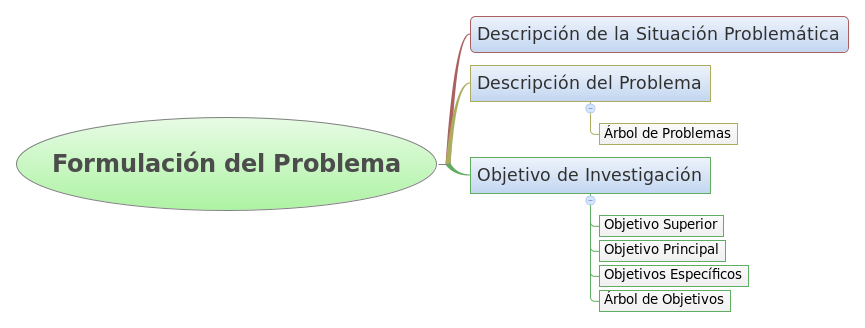
\includegraphics[scale=0.60]{./img/MapaMental/capitulo02.png}
	\caption{Mapa Mental del Cap�tulo de Formulaci�n del Problema}
	\label{Mapa Mental del Capitulo de Formulaci�n del Problema}
\end{figure}


\section {Descripci�n de la situaci�n problem�tica}
\label{section.Descripcion.de.la.situacion.problematica}

El proyecto OLPC pretende ser una apuesta por el uso de laptops de bajo coste para disminuir la brecha digital. Los componentes que instrumentalizan este proceso son el software y el proceso educativo.
La falta de informaci�n sobre la usabilidad del software del escritorio gr�fico SUGAR del proyecto de las OLPC es una inquietud que impacta en la aceptaci�n de esta propuesta. El evaluador generalmente es un grupo de adultos con conocimiento de plataformas mayoritariamente usadas\footnote{Colocar Nota sobre plataformas de software mas usadas.}, y la inclusi�n de SUGAR y linux dentro del proyecto OLPC cre� un ambiente de incredulidad sobre lo viable de su propuesta\footnote{Daniel Wagner, profesor de la Escuela de Graduaci�n en Educaci�n de la Universidad de Pensilvania, a�ade que son pocas las investigaciones que establecen una relaci�n directa entre el uso del port�til en el aula y el avance educativo. Karl Ulrich, profesor de Gesti�n de la Informaci�n y Operaciones, y Andrea Matwyshyn, profesora de Estudios Jur�dicos, dicen que el abaratamiento de la tecnolog�a de la computaci�n puede llevar al desarrollo econ�mico. Eric Clemons, profesor de Gesti�n de la Informaci�n y Operaciones, cuestiona si un aparato de 100 d�lares -precio inicial de la m�quina de OLPC� ser�a efectivamente barato. Harry Brignull Creativity is of course very important, but it has to be tempered within the requirements of the target audience. 
Fuente:
http://www.90percentofeverything.com/2006/11/23/why-the-olpc-needs-lots-of-usability-work/ 

http://wharton.universia.net/index.cfm?fa=viewArticle\&ID=1535 16/02/2009 }. 


% ----------------------------------------------
\section {Descripci�n del Problema}
\label{section.Descripcion.del.Problema}

La OLPC es un producto con varios conceptos novedosos. El primero es otorgar una laptop a cada ni�o para disminuir la brecha digital con el uso de tecnolog�a en el aula. El segundo es el uso de linux con un escritorio gr�fico no convencional SUGAR\footnote{Se refiere a convencional a los escritorios parecidos en interfaces a Windows o Linux} este escritorio presenta un conjunto de programas educativos o \textbf{Actividades}  que apoyar�n a los ni�os y docentes en el proceso educativo. El desarrollo, al inicio, de una comunidad de colaboradores para apoyar la viabilidad del proyecto.
A�n as� el proyecto recibi� severas cr�ticas que continuaron acentu�ndose con el paso del tiempo. The Economist aclara, algunos problemas en la implementaci�n del OLPC han terminado con el laptop transform�ndose en un mal producto tecnol�gico, a pesar de los avances a los que ha contribuido. B�sicamente, estos problemas se reducir�an a dos: la usabilidad de la tecnolog�a\footnote{Fuente: www.economist.com/daily/columns/techview/displaystory.cfm?story\_id=10472304 Tech.view Jan 4th 2008 . 02/02/2009} (empezar desde cero en vez de aprovechar los avances en la materia) y la falta de documentaci�n y otros m�todos para integrar los laptops en las escuelas, en el entrenamiento de los profesores, etc. Otra cr�tica en torno a este tema fu� en un art�culo de BusinessWeek\footnote{Fuente:http://www.businessweek.com/innovate/content/mar2007/id20070301\_063165.htm. March 1, 2007 . The Face of the \$100 Laptop by Steve Hamm. 10/10/2009  }, Jakob Nielsen\footnote{http://www.useit.com/jakob/ 20/10/2009} llama el enfoque de dise�o de interfaz de usuario OLPC imprudente porque no han hecho pruebas de usuario hasta el momento.
El proyecto OLPC al ser un proyecto que pretende amplitud social se complejiza en otras �reas fuera del tecnol�gico surgiendo interrogantes que escapan al estudio pero son v�lidas de se�alarlas: 

\textbf{-} �Cu�l es la concepci�n del Conocimiento detr�s del OLPC?
	
\textbf{-} �C�mo se construye el Conocimiento con un dispositivo como el del OLPC? 
	
\textbf{-} �C�mo el OLPC afecta la relaci�n de poder entre los profesores y los ni�os?
	
\textbf{-} �En qu� medida el OLPC afecta la subjetividad de los ni�os y la institucionalidad de la Escuela? 
	
\textbf{-} �Da lo mismo usar un sistema operativo abierto que cerrado en el OLPC?

\begin{figure}[ht]
		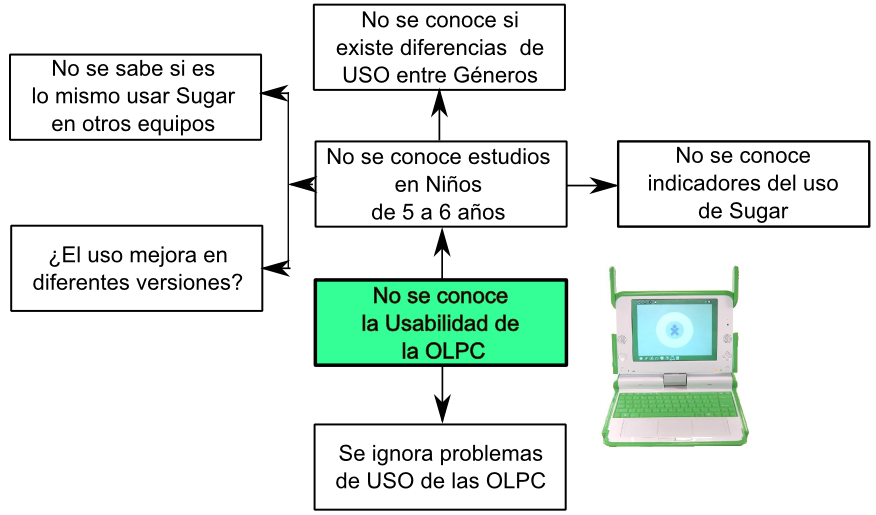
\includegraphics[width=0.70\textwidth]{./img/arboldeProblemas1.png}
	\caption{�rbol de Problemas}
	\label{ArboldeProblemas}
\end{figure}

Desglozando el �rbol de problemas se tiene lo siguiente:

\textbf{-} No se conoce la Usabilidad de la OLPC.

\textbf{-} Se ignora problemas de USO de las OLPC.

\textbf{-} No se conoce indicadores del uso de Sugar.

\textbf{-} No se conoce estudios en Ni�os de 5 a 6 a�os.

\textbf{-} No se conoce si existe diferencias de USO entre G�neros.

\textbf{-} No se sabe si es lo mismo usar Sugar en otros equipos.

\textbf{-} �El uso mejora en diferentes versiones?.



% ----------------------------------------------
\section {Objetivo de la Investigaci�n}
\label{section.Objetivo.de.la.Investigacion}

\subsection{Objetivo Superior}
\label{subsection.Objetivo.Superior}
Contar con un estudio cuantitativo que contraste la usabilidad del software del escritorio SUGAR de la laptop XO OLPC. Para el estudio se utilizar� el m�todo de la Prueba de Usabilidad.

\subsection{Objetivo Principal}
\label{subsection.Objetivo.Principal}
\textbf{O.0} Conocer la Usabilidad. Y medir la Usabilidad utilizando Pruebas de Usabilidad y m�tricas cuantitativas. 

\subsection{Objetivos Espec�ficos}
\label{subsection.Objetivos.Especificos}

\textbf{- O.1} Usar Pruebas de Usabilidad con Ni�os de 5 a 6 a�os: Formalmente la Prueba debe obtener informaci�n de la interacci�n de las  interfaces de Sugar.

\textbf{- O.2} Conocer la Usabilidad de Sugar por G�nero: Se tiene informaci�n de desarrollo diferentes de acuerdo al tipo g�nero se buscar� comprobar esta afirmaci�n.

\textbf{- O.3} Encontrar M�tricas de la Usabilidad de Sugar: Intentar usar propuestas formales para encontrar indicadores sobre el Uso de Sugar.

\textbf{- O.4} Comparar la Usabilidad entre versiones de Sugar: Es posible que las mejoras resulten propuestas sin retroalimentaci�n. Se buscar� conocer con las pruebas el estado asertivo del control de las versiones.

\textbf{- O.5} Conocer la Usabilidad de Sugar en otros Equipos: Usar Sugar en otros dispositivos competidores de la OLPC y conocer su usabilidad en ellos.

\textbf{- O.6} Reconocer posibles problemas de Uso y Mejorar: Conocer posibles problemas de ergonom�a, dise�o de interfaces. Por lo menos plantear propuestas de mejora.


%A continuaci�n se describen los �rboles de problemas y objetivos para puntualizar el la motivaci�n de la tesis y su propuesta.

%\subsection{�rbol de Problemas}
%\label{subsection.Arbol.de.Problemas}


%Desglozando se obtiene la siguiente jerarqu�a de problemas:
%\begin{enumerate}
%	\item No se conoce la Usabilidad de la OLPC.
%	\item No se conoce estudios en Ni�os de 5 a 6 a�os.
%	\item No se conoce si existe diferencias de USO entre G�neros.
%	\item No se conoce indicadores del uso de Sugar.
%	\item �El uso mejora en diferentes versiones?.
%	\item No se sabe si es lo mismo usar Sugar en otros equipos.
%\end{enumerate}

\subsection{�rbol de Objetivos}
\label{subsection.Arbol.de.Objetivos}


De los propuesto en la sessi�n \ref{subsection.Objetivos.Especificos} y \ref{subsection.Objetivo.Principal} se puede elaborar el siguiente �rbol de Objetivos:

\begin{figure}[ht]
	\centering
		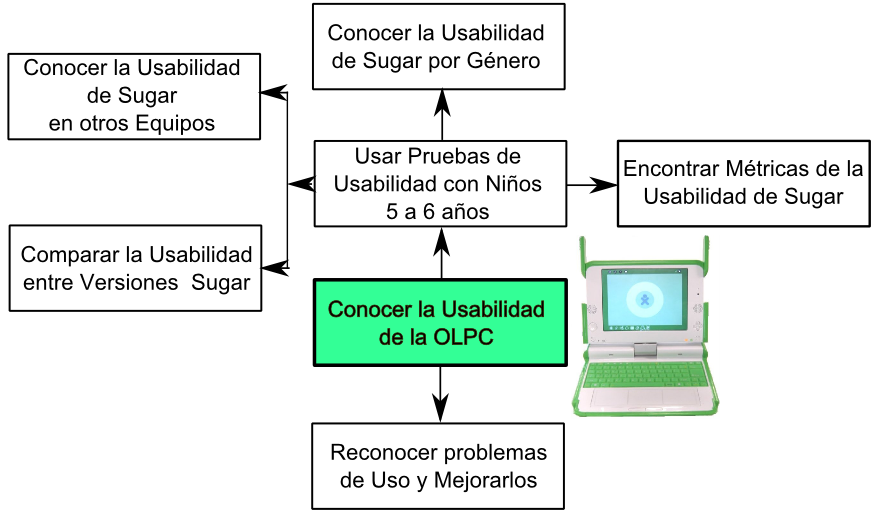
\includegraphics[width=0.70\textwidth]{./img/arboldeObjetivos1.png}
	\caption{�rbol de Objetivos}
	\label{ArboldeObjetivos}
\end{figure}


 %2. Formulaci�n del Problema
%\chapter{MARCO TE�RICO}
%\vspace*{8cm}
\chapter{Marco Te�rico}
\label{chapter.Marco.Teorico}
% ----------------------------------------------

\begin{figure}[ht]
	\centering
		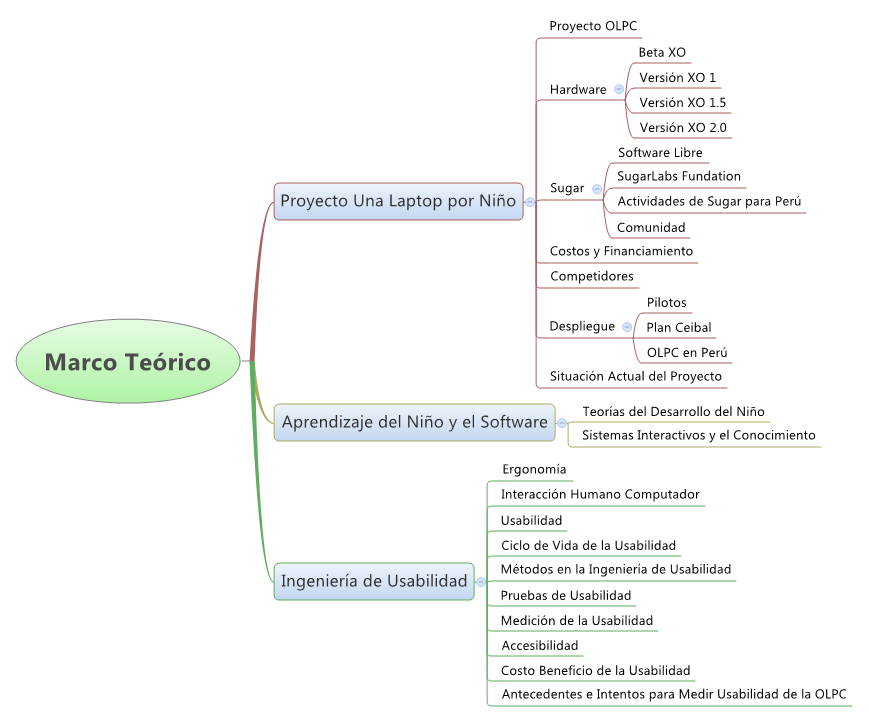
\includegraphics[scale=0.5]{./img/MapaMental/capitulo03.png}
	\caption{Mapa Mental del Cap�tulo de Marco Te�rico}
	\label{Mapa Mental del Capitulo de Marco Te�rico}
\end{figure}


\section{Proyecto Una Laptop por Ni�o}
\label{section.Proyecto.Una.Laptop.por.Ninhio}

Se referir� al proyecto Una Laptop por Ni�o o One Laptop for Child con las siglas OLPC.

\subsection{Proyecto OLPC}
\label{section.Proyecto.OLPC}
% ----------------------------------------------
\subsubsection{Misi�n}
\label{subsection.Mision}

\subsubsection{Alianzas}
\label{subsection.Alianzas}

\subsubsection{Cronolog�a}
\label{subsection.Cronologia}

\subsection {Costos y Financiamiento}
\label{section.Costos.y.Financiamiento}
% ----------------------------------------------

\subsubsection{Estructura de Costos}
\label{subsection.Estructura.de.Costos}

PCs de bajo costo son una tendencia en los mercados emergentes, como la penetraci�n de PC es baja. Pero eso no significa que los vendedores de PC puede ignorar todo, excepto los costes. EL proyecto OLPC caus� interes justamente en el costo de sus equipos. Se muestra en el cuadro \ref{EstructuraDeCostos} es un desglose de los costos de fabricaci�n de la OLPC extraido del an�lisis OLPC. Another blue sea or a bubble? de Merrill Lynch\cite{Merrill}(2007).

\begin{table}[ht]
	\centering
		\begin{tabular}{|m{7cm}|m{2cm}|}
			\hline
			Componente y Especificaci�n & Precio \\\hline
			CPU: AMD Geodo Gx2 500
		
			Chipset: Integrado &  28 \\\hline 
			Memoria: 128MB DDR266	&  10 \\\hline
		  Panel: 7.5 dual model TFT &  28 \\\hline
		  Disco: 512 MB SLC NAND flash &  8 \\\hline
		  Wifi: 802.11b/g (Marvell) &  5 \\\hline
		  OS: Linux y otros. &  10 \\\hline
		  Bater�a: 5 cells (NiMH) & 7 \\\hline
		  Otros:  & 44 \\\hline
		  \textbf{Sistema de Costo}  & \textbf{140} \\\hline		  
		  \textbf{Precio en Calle}  & \textbf{150} \\\hline
		\end{tabular}
	\caption{Estructura de Costos. Fuente Compa�ias y estimaci�n de Merrill Lynch}
	\label{EstructuraDeCostos}
\end{table}



\subsubsection{Referencias del Costo de Implantaci�n}
\label{subsection.Referencias.del.Costo.por.Implantacion}

Se muestra un estudio sobre los costos de implantaci�n del proyecto de OLPC uno extraido del portal de Olpcnews\footnote{Fuente: www.olpcnews.com/sales\_talk/price/the\_real\_cost\_of\_the.html 12/05/2008}.
Los costos de implantaci�n est�n proyectados para un plazo de 5 a�os \ref{Costos.de.la.implantacion.del.Proyecto.OLPC.por.5.Anhios}

\begin{table}
\centering
\begin{tabular}{|m{5cm}|m{2cm}|}
\hline
\multicolumn{2}{|m{7cm}|}{Costos por LAPTOP en 5 A�os}\\
\hline
Instalaci�n  & ~ \\\hline
Hardware Inicial &  \$/.148.00 \\\hline
Instalaci�n Primera Vez & \$/. 108.00 \\\hline
\textbf{Total}  & \$/. \textbf{256.00} \\\hline
Entrenamiento & ~ \\\hline
Anual &  \$/. 27.60 \\\hline
\textbf{Total Entrenamiento} & \textbf{\$/. 138.00} \\\hline
Mantenimiento & ~ \\\hline
Anual & \$/. 7.40 \\\hline
\textbf{Total Mantenimiento} & \textbf{\$/. 37.00} \\\hline
Internet  & ~ \\\hline
Primer A�o \$1  &   \$/. 1.00\\\hline
Anual &  \$/. 135.00\\\hline
\textbf{Total Internet}  & \textbf{\$/. 541.00} \\\hline
\textbf{Costo Total en 5 A�os}  & \textbf{\$/. 972.00} \\\hline
\end{tabular}
\caption{Costos de la implantaci�n del Proyecto OLPC por 5 A�os}
\label{Costos.de.la.implantacion.del.Proyecto.OLPC.por.5.Anhios}
\end{table}

Se nota que se tendr�a un costo por el valor de \$/.972 dolares .


\subsection{Despliegue}
\label{section.Despliegue}


\begin{table}[ht]
\centering
\footnotesize
\begin{tabular}{|m{2cm}|m{0.5cm}|m{0.5cm}|m{0.5cm}|m{0.5cm}|m{0.5cm}|m{0.5cm}|m{0.5cm}|m{0.3cm}|m{0.3cm}|m{0.3cm}|m{0.3cm}|m{0.3cm}|m{0.3cm}|}
\hline
{\bf Actividades } & C.I & L.M & P.S & C.A & E.A & E.F & E.R & 1� & 2� & 3� & 4� & 5� & 6� \\\hline
Escribir & X & X & X & X & X & X & X &   & X & X & X & X & X \\\hline
Navegar & X & X & X & X & X & X & X &   &  & X & X & X & X \\\hline
Charla & X & X & X & X & X & X & X &   &  & X & X & X & X \\\hline
Record & X & X & X & X & X & X & X & X & X & X & X & X & X \\\hline
Pintar & X & X & X & X & X & X & X & X & X & X & X & X & X \\\hline
TortugArte &  & X &  &  &  &  &  &  &  & X & X & X & X \\\hline
TamTamJam &  &  &  &  & X &  &  & X & X & X & X & X & X \\\hline
Etoys &  &  &  &  & X &  &  &  &  & X & X & X & X \\\hline
Pippy &  & X &  &  &  &  &  &  &  &  & X & X & X \\\hline
Calculadora &  & X & X & X &  & X &  & X & X & X & X & X & X \\\hline
Juego de memoria & X & X & X & X & X & X & X & X & X & X & X & X & X \\\hline
Juego 4 en l�nea & X & X &  &  &  &  &  &   & X & X & X & X & X \\\hline
Regla &  & X & X & X &  & X &  & X & X & X & X & X & X \\\hline
Acoustic &  & X & X & X &  & X &  &   & X & X & X & X & X \\\hline
Clock &  & X &  & X &  & X &  & X & X & X & X & X & X \\\hline
Stopwatch &  &  &  &  &  & X &  & X & X & X & X & X & X \\\hline
Tan gram & X & X &  &  &  & X &  & X & X & X & X & X & X \\\hline
Scratch & X &  & X &  &  & X &  &   &  &  & X & X & X \\\hline
Implode &  & X &  &  &  &  &  &   & X & X & X & X & X \\\hline
Maze & X & X & X & X & X & X &  & X & X & X & X & X & X \\\hline
Jigsaw puzzle & X & X & X & X & X & X & X & X & X & X & X & X & X \\\hline
Speak & X & X & X & X & X & X & X & X & X & X & X & X & X \\\hline
Scalesboard & X & X & X & X &  & X &  &  & X & X & X & X & X \\\hline
Sudoku & X & X & X &  &  & X &  &   & X & X & X & X & X \\\hline
Terminal & X & X & X & X &  & X &  &   &  &  & X & X & X \\\hline
Moon (Luna) & X &  & X & X &  & X &  & X & X & X & X & X & X \\\hline
\end{tabular}  
\caption{Actividades vs �reas de Aprendizaje}
\label{ActividadesvsAreasdeAprendizaje}
\end{table}


\subsubsection{Perspectivas Sobre el Desarrollo del Ni�o}
\label{subsection.Perspectivas.Sobre.el.Desarrollo.del.Ninhio}
Kail\cite{Kail} (2002) identifica cinco perspectivas te�ricas en el desarrollo del ni�o: biol�gico, psicodin�mico, aprendizaje, desarrollo cognitivo, y contextuales. 

\textbf{Biol�gico}
\label{subsubsection.Biologico}
Las teor�as que tienen una perspectiva biol�gica dejan de lado los factores externos, las personas y los eventos tienen poco o ning�n efecto sobre los ni�os en su desarrollo. Una de esas teor�as la teor�a de la madurez (Arnold Gesell\footnote{Arnold Lucius Gesell 1880-1961, psic�logo y pediatra estadounidense. Pionero en investigar el crecimiento y pensamiento del ni�o desde su nacimiento.},  sostiene que los ni�os se desarrollan independientemente del contexto. Otra teor�a etol�gicas asume que la experiencia poco impacto. Konrad Lorenz\footnote{Konrad Lorenz nacio el  7 Noviembre de 1903 en Austria. Premio Nobel de Psicolog�a y Medicina y fundador de la etolog�a.} apoy� este punto de vista al afirmar que el aprendizaje s�lo puede tener lugar si ocurre en ese momento.

\textbf{Psicodin�mico}
\label{subsubsectionPsicodinamico}
Esta perspectiva sobre el desarrollo del ni�o incluye las obras de Sigmund Freud\footnote{Sigmund Freud (1856-1939). Naci� en Moravia, una regi�n de la actual Rep�blica Checa. M�dico y neur�logo austriaco, fundador del psicoan�lisis.} y su alumno Erik Erikson\footnote{Erick Erickson (1902-1994). Fue un psicoanalista Alem�n nacionalizado estadounidense que postul� la Teor�a del Desarrollo del Ni�o. Sostuvo que los ni�os se desarrollan en un orden predeterminado.}. Freud ofrece un trabajo esencialmente sobre la teor�a de la personalidad definida en tres comnponentes.  

\textbf{- }Id (Instintos Primitivos) 

\textbf{- }Ego (El comportamiento racional) 

\textbf{- } SuperEgo (El componente moral) 

Estos cuentan con el apoyo de una teor�a del desarrollo psicosexual que sostiene que el desarrollo se produce mejor cuando el ni�o y sus necesidades se cumplan. Erikson se centro en los aspectos sociales del desarrollo, y se produjo una teor�a psicol�gica que una persona en toda la vida se divide en ocho etapas, cada una con sus propios desaf�os. Erikson trabajo, no s�lo sobre los ni�os, sino que considera a la  persona en toda su vida. Las etapas en los ni�os son muestran en la Tabla \ref{Teoria.de.Erikson}. 

  
% ---------------------------------
\subsection{Usabilidad} 
\label{section.Usabilidad}

\subsubsection{�Qu� es la Usabilidad?} 
\label{section.Que.es.la.Usabilidad}

El t�rmino usabilidad es extensamente utilizado y muchas son los conceptos que intentan definirlos. Por ejemplo, Guillemette (1989)\cite{Guille} conceptualiza la usabilidad en torno al uso de documentaci�n.
Identificando conceptos de eficacia y satisfacci�n del usuario, se nota una relaci�n entre conceptos de usabilidad y utilidad. As� mismo la norma la Organizaci�n Internacional de Est�ndares (OSI u ISO) expone dos normas ISO la 9126 y 9241 orientadas al producto software de las se desprenden dos conceptos diferentes usabilidad sujetos a su contexto de desarrollo. 

Por lo tanto un concepto de usabilidad no existe en ning�n sentido absoluto, sino que s�lo puede definirse con referencia a determinados contextos\footnote{Esto, a su vez, significa que no hay absolutas medidas de usabilidad, ya que, si la usabilidad de un artefacto es definida por el contexto en el que tal artefacto se utiliza, medidas de usabilidad debe necesariamente ser definido por ese contexto.}. A pesar de ello, existe la necesidad de medidas de car�cter general que puede ser usado para comparar la usabilidad a trav�s de una variedad de contextos. Adem�s, existe la necesidad de pruebas r�pidos e informales de bajo costo para permitir la evaluaci�n de la usabilidad en los sistemas industriales.

\subsubsection{Preparaci�n de Materiales}
\label{subsection.Preparacion.de.Materiales}

Las pruebas de usabilidad se dan en ambientes f�sicos y virtuales. Para las pruebas llevadas acabo en ambientes virtuales se pueden caracterizar por tener sistemas online que ejecutan ciertas acciones de acuerdo a las actividades del usuario a�n si este no tenga conciencia que su actividad est� siendo monitoreada. En esta secci�n no se detallar� sobre pruebas de usabilidad remotas, virtuales o en l�nea orientadas a generalmente a software de internet, p�ginas o aplicativos web. Las pruebas de usabilidad presenciales son divididas en pruebas de campo y pruebas en laboratorio. Ambas pruebas necesitan la rigurosa tarea de estar detalladas en un Plan de Pruebas, en tanto estas deben ser tomadas en ambientes que permitan al participante tener atenci�n durante la prueba. Inclusive para pruebas con juguetes o artefactos cuya utilidad necesite estar interactuando en el contexto de su objetivo, las pruebas de campo ser�n la soluci�n mas coherente para medir la respuesta de los usuarios ante un evento com�n de uso(simuladores de vuelo, clases escolares, operaciones m�dicas).

\begin{table}[ht]
	\centering
	\footnotesize
		\begin{tabular}{|m{3.5cm}|m{8cm}|}
		\hline
\textbf{Equipo B�sico}& PC or laptop.

Software de Grabaci�n.

Software Biom�tricos.

Webcam o Camera de Video.\\\hline	
\textbf{Formularios y Herramientas a Tomar Notas}& Grabador de Audios.

Convenio de No Divulgaci�n(Si Fuese Necesario).

Formularios de Consentimiento.

Cuestionarios.

Resumen de las caracter�sticas de los participantes.

Script de Sesiones.

Escenarios Para los Participantes.

Instrucciones para los Observadores.

Calendario de Sesiones.

Recibos para Honorarios.\\\hline	
\textbf{Artefactos}&Prototipo de las pruebas.

Los n�meros de cuenta.

ID de usuario y contrase�as.

Datos falsos u otros elementos para hacer realista las pruebas.\\\hline	
		\end{tabular}
	\caption{Materiales de las Pruebas de Usabilidad}
	\label{MaterialesdelasPruebasdeUsabilidad}
\end{table}


\subsubsection{Estad�stica para las M�tricas}
\label{subsection.EstadisticaparalasMetricas}
Para desarrollar un an�lisis cuantituativo con los resultados de las pruebas de usabilidad se tendr�n encuenta algunas estad�sticas:


\textbf{1. Estad�stica Descriptiva:} Son esenciales para cualquier intervalo o relaci�n de datos. 

\textbf{- }Medidas de tendencia central: Son la primera cosa que debe buscar cuando se ejecuta la estad�stica descriptiva. Tendencia central es simplemente la media de cualquier distribuci�n. 

\textbf{- }Medidas de Variabilidad: Muestra como los datos est�n repartidos o dispersos. Estas medidas ayudar�n a responder la pregunta: �La mayor�a de datos tiende a... ?.

\textbf{- }Intervalos de confianza: Son sumamente valiosos para cualquier profesional de la usabilidad. Un intervalo de confianza es una gama de estimaciones del verdadero valor de una poblaci�n estad�stica. 

\textbf{2. Comparando medias:} Una de las cosas m�s �tiles que puedes hacer con intervalo o relaci�n de datos para comparar diferentes medias. 

\textbf{- }Muestras Independientes: Frecuentes en estudios de usabilidad est� comparando medios basados en muestras independientes. 
	
\textbf{- }Muestras Dependientes: Muestras apareadas se usan la prueba t. 

\textbf{3. Relaciones Entre las Variables:} A veces es importante saber acerca de la relaci�n entre los diferentes participantes variables. Cuando se le pidi� que la tasa de lo f�cil o dif�cil que era.

\textbf{- }Correlaciones: La primera vez que comenzar a examinar la relaci�n entre dos variables, es importante visualizar lo que los datos parecen. 


\textbf{4. Pruebas No Param�tricas:} De utilizan para el an�lisis de datos nominales y ordinales. Por ejemplo, es posible que desee saber si existe una diferencia significativa entre hombres y mujeres para el �xito y el fracaso en una tarea en particular. 

\textbf{- }La prueba de Chi-Cuadrado: Se utiliza cuando se quiere comparar de datos de categorias o nominales.


Estos resultados se pueden cruzar en o que ser�a una Tabla de Confianza de Datos.



% ---------------------------------
\subsection{Costo Beneficio de la Usabilidad}
\label{section.Costo.Beneficio.de.la.Usabilidad}


\subsubsection{An�lisis del Costo Beneficio}
\label{susection.Analisis.del.Costo.Beneficio}
Una ingenier�a de usabilidad an�lisis coste-beneficio se lleva a cabo en el proceso de desarrollo de software por dos razones principales:

\textbf{1. }Para demostrar la facilidad de uso que la ingenier�a es viable y un importante ahorro de costes enfoque.

\textbf{2. }Para planificar el programa de ingenier�a de usabilidad para un proyecto de desarrollo.

En m�s detalle que la prevista en la presente rese�a se hace referencia a Mayhew\cite{CJUsability}.

\textbf{- }Varios tipos de tareas se incluyen en el Ciclo de Vida de Ingenier�a de Usabilidad, de la siguiente manera:

\textbf{- }Estructurado el an�lisis de los requisitos de usabilidad tareas.

\textbf{- }Un objetivo expl�cito de usabilidad establecimiento tarea, impulsada directamente de los requisitos de n�lisis de datos.

\textbf{- }Tareas de apoyo a una estructura, de arriba hacia abajo para el dise�o de interfaz de usuario que es impulsada directamente desde la usabilidad objetivos y requisitos de datos.

\textbf{- }Objetivo facilidad de uso para las tareas de evaluaci�n de dise�o iterando hacia objetivos de la usabilidad.


\begin{center}
\begin{longtable}{|m{2.5cm}|m{11cm}|}
 \hline
  \textbf{Item }& \textbf{Comentario}\\
  \hline
\endfirsthead
  \hline
%  \textbf{Item} & \textbf{Comentario}\\
%  \hline
%\endhead
%\hline
\caption{Beneficio Econ�mico de la Usabilidad}
\label{Beneficio.Economico.de.la.Usabilidad}
\endlastfoot
\hline
\multicolumn{2}{|m{13.5cm}|}{Beneficio Econ�mico de la Usabilidad}\\
%\hline
%\endfoot
%\footnotetext{Pie de P�gina del Cuadro de Beneficio Econ�mico de la Usabilidad}
\hline
%& \\\hline
\multicolumn{2}{|m{13.5cm}|}{\bfseries Valor global en la aplicaci�n con  las pr�cticas de la interfaz de usuario }\\\hline
Alto rendimiento, ahorros y productos usables & Una vez que un sistema est� en desarrollo, corregir un problema cuesta 10 veces m�s que la fijaci�n del mismo problema en el dise�o. Si el sistema ha sido puesto en libertad, que cuesta 100 veces m�s en relaci�n a la fijaci�n de dise�o, GILB, 1988 \cite{GILB}.\\\hline
\multicolumn{2}{|m{13.5cm}|}{\bfseries Desarrollo: Reducir los Costos}\\\hline
Preservar los costos de desarrollo & Aproximadamente el 63 porciento de los grandes proyectos de software se exceden en su presupuesto y las cuatro principales razones cr�ticas est�n relacionadas con la ingenier�a de usabilidad, Nielsen, 1993 \cite{UsabilityE}.\\\hline
Preservando el tiempo en desarrollo & Acelerar el desarrollo es un objetivo clave para la integraci�n de la usabilidad de manera efectiva en el desarrollo de productos; una cuarta parte de lo que demora un producto en el mercado puede resultar en la p�rdida del 50 porciento de los beneficios del producto, Conklin, 1991 \cite{Conklin}. \\\hline
Reducir el costo de mantenimiento & Se ha constatado que el 80 porciento de los costos del software de su ciclo de vida se producen durante la fase de mantenimiento y se asociaron necesidades insatisfechas o imprevistas de los usuarios y otros problemas de usabilidad (Nielsen, 1993)\cite{UsabilityE}.\\\hline
Evitando el Costo en Redise�o & En Microsystems ha demostrado el gasto de alrededor de 20.000 d�lares podr�a producir un ahorro de 152 millones de d�lares. Cada d�lar invertido podr�a dirigirse en 7500 d�lares de ahorro, Rhodes \footnote{Fuente: www.webword.com/moving/savecompany.html 19/02/2009}.\\\hline
\multicolumn{2}{|m{13.5cm}|}{\bfseries Ventas: Aumentar los Ingresos}\\\hline
Aumentar las transacciones / compras & Usted puede aumentar las ventas en su sitio tanto como 225 porciento mediante el suministro de suficiente informaci�n sobre el producto a sus clientes en el momento adecuado (User Interface Engineering)\footnote{Fuente:  www.uie.com/ 19/02/2009}.\\\hline
Aumentar las Ventas de Productos & Es com�n que los esfuerzos en la usabilidad resulten en un cien por ciento o m�s de aumento en el tr�fico de ventas (Nielsen, 1999)\cite{Niel4}\\\hline
Incremento de Tr�fico, tama�o de audiencia & IBM dice que en febrero 1999 un mes despu�s del re-lanzamiento de la tienda en l�nea de IBM el tr�fico aumento de 120 porciento, y las ventas subieron 400 porciento, Battey, 1999 \footnote{Battey, J. (1999). IBM Redesign Results in a Kinder, Simpler Web Site. Fuente: www.infoworld.com/cgi-bin/displayStat.pl?/pageone/opinions/hotsites/
hotextr990419.htm 19/02/2009.}. El cambio en las interfaces pueden significar el aument� del tr�fico en mas de porciento.\\\hline
Retener clientes & M�s del 83 porciento de los usuarios de Internet es probable que deja un sitio Web si se sienten que tienen que hacer demasiados clics para encontrar lo que est�s buscando\footnote{Arthur Andersen. Web Site Design Survey.}.	\\\hline
Aumentar la cuota de mercado (ventaja competitiva) & La importancia de tener una ventaja competitiva en la facilidad de uso puede ser incluso m�s pronunciada para los sitios de comercio electr�nico, lo que com�nmente en conduce a cerca de la mitad de las empresas es repetir lo que hace dif�cil para los visitantes: Encontrar la informaci�n que necesitan\footnote{Manning, H. The right way to test ease-of-use. In G. M. Donahue, S. Weinschenk, and J. Nowicki, Usability Is Good Business. Fuente: www.compuware.com 19/02/2009}.\\\hline
\multicolumn{2}{|m{13.5cm}|}{\bfseries Uso: mejorar la eficacia}\\\hline
Incrementar la tasa de �xito, reducir los errores de los usuarios & En el estudio de Jared Spool\footnote{Jared M. Spool investigador de interfaces gr�ficas. Fundador de User Interface Engineering} de 15 grandes sitios comerciales los usuarios pueden encontrar informaci�n el 42 porciento del tiempo, aun despu�s de corregir el home page antes que ellos realizaran las tareas de la prueba\footnote{Nielsen, Jackob. Failure of Corporate Websites. Fuente: www.useit.com/alertbox/981018.html 19/02/2009}).\\\hline
Atraer m�s clientes & Cuando se pregunt� a los encuestados a la lista de cinco razones m�s importantes para comprar en la web, el 83 porciento dijo: F�cil de colocar una orden como la raz�n principal, Nielsen \cite{Niel4}.\\\hline
Aumentar la eficiencia / productividad (reducir el tiempo para completar tareas) & La falta de utilizaci�n de m�todos de ingenier�a de usabilidad en proyectos de desarrollo de software se han estimado en costos a la econom�a de los EE.UU. en alrededor de 30 mil millones de d�lares por a�o en p�rdida de productividad, Landauer, 1997 \cite{Landa}.\\\hline
Aumentar la satisfacci�n de los usuarios & En un estudio de Gartner Group, los m�todos de usabilidad planteadas con puntuaciones de satisfacci�n de los usuarios en un sistema con un 40 porciento, cuando los sistemas deben coincidir con las necesidades de los usuarios, la mejora la satisfacci�n a menudo fue manera espectacular, Harrison, 1994 \cite{Harris}.\\\hline
Incrementar la tasa de �xito, reducir los errores de los usuarios & Encuestas muestran que las pantallas de video en las terminales de trabajo tienen el doble de quejas en dolores de hombros acompa�ado en dolores de cuello, cansancio de visual reportado tres veces mas que otras, junto con altas tasas de absentismo, menos satisfacci�n en el trabajo y aumento en un 30 porciento de la carga laboral. Schneider, 1985 \cite{Schne}.\\\hline
Aumenta la facilidad de Uso & La incorporaci�n de la facilidad de uso en sus productos realmente ahorra dinero. Informes muestran que es m�s econ�mico para examinar las necesidades de los usuarios en las primeras etapas de dise�o, que resolverlas m�s adelante \footnote{IBM. Cost Justifying Ease of Use: Complex Solutions Are Problems. Fuente: from www-3.ibm.com/ibm/easy/eou\_ext.nsf/Publish/23 19/02/2009}.\\\hline
Aumenta la facilidad de Aprendizaje & Un estudio realizado por Computer + Software News (1986) encontraron que los usuarios evaluados sobre la facilidad de usose eleva al doble en 6,8 de cada 10, mientras que la facilidad de aprendizaje fue elevado sobre cuarto en 6,4 y son  factores importantes para la compra\cite{Harris}.\\\hline
Aumentar la confianza en los sistemas & [EuroClix]... el estudio muestra claramente que la confianza en los consumidores aumenta y las preocupaciones pueden ser aliviadas mediante el suministro de informaci�n pertinente cuando y donde los usuarios lo necesitan, Egger, 2000 \cite{Egger}.\\\hline
Diminuye los costos de soporte & En la pr�xima versi�n, las llamadas al soporte t�cnico carer�n dram�ticamente; Microsoft reconoce importantes ahorros en costes, Ehrlich, 1994 \cite{Ehrli} . M�s de 50.000 usuarios han llamado al centro de asistencia, a un costo a la empresa de casi  500.000 d�lares al mes. Para corregir esta situaci�n, el fabricante... termin� gastando 900.000 d�lares en el problema. No se realiz� ninguna prueba de usuario... antes de esta versi�n.\\\hline
Reduce la capacitaci�n / costo de documentaci�n & Un estudio realizado por Computer + Software News (1986) encontr� que el manejo de los sistemas de informaci�n evaluados por su facilidad con una valoraci�n de 7 (de 10) en la escala es un importante factor para su compra\cite{Harris}.\\\hline
\multicolumn{2}{|m{13.5cm}|}{\bfseries Otros}\\\hline
Responsabilidad de la disuasi�n y la seguridad & Usabilidad es un factor principal para determinar los fabricantes la responsabilidad de expertos sobre la base de pruebas fehacientes sobre la forma de un dise�o deber�a haber utilizado la usabilidad.\\\hline
\end{longtable}
\end{center}


% ---------------------------------
\subsection{Antecedentes e Intentos para Medir Usabilidad de la OLPC}
\label{section.Antecedentes.e.Intentos.para.Medir.Usabilidad.de.la.OLPC}


 %3. Marco Teorico
%\chapter{INVESTIGACI�N}
%\vspace*{8cm}
\chapter{Investigaci�n}
\label{Metodologia.de.la.Investigacion}

\begin{figure}[ht]
	\centering
		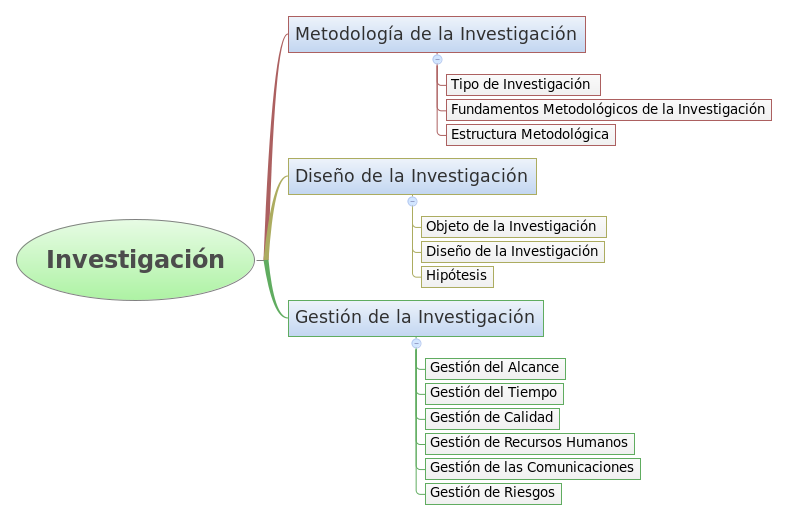
\includegraphics[scale=0.55]{./img/MapaMental/capitulo04.png}
	\caption{Mapa Mental del Cap�tulo de Investigaci�n}
	\label{Mapa Mental del Capitulo de Investigaci�n}
\end{figure}


\section{Metodolog�a de la Investigaci�n}
\label{chapter.Metodologia.de.la.Investigacion}
% ----------------------------------------------

En este cap�tulo se detalla la metodolog�a de la investigaci�n su fundamento y tipo de metodolog�a.

\subsection{Tipo de Investigaci�n}
\label{section.Tipo.de.Investigacion}

La investigaci�n desarrollada es una investigaci�n del tipo exploratorio, correlacional y de campo presentada dentro de un ambiente de implantaci�n del Programa de Una Laptop por Ni�o\ref{section.OLPC.en.Peru}. Donde se encuentra varias variables como dominio que necesitan ser relacionadas para formar parte del rango de las buenas pr�cticas.


\subsection{Estructura Metodol�gica}
\label{section.Estructura.Metodol�gica}

Escapa de la tesis de grado detallar y redundar tecnicas sobre la elaboraci�n de una metodolog�a que envuelva la elaboraci�n de la investigaci�n, sin embargo en la Figura \ref{MetodologiaInvestigacion}
se presenta un esquema de la metolog�a de investigaci�n.

\begin{figure}[ht]
	\centering
		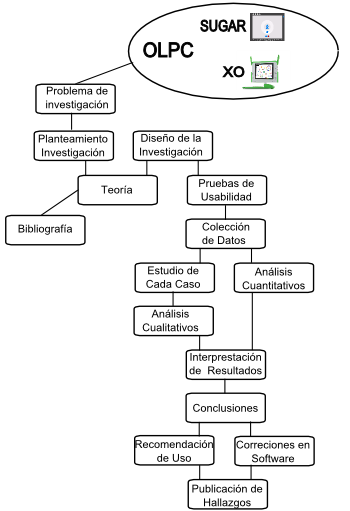
\includegraphics[scale=0.6]{./img/MetodologadelaTesis.png}
	\caption{Metodolog�a para la Tesis}
	\label{MetodologiaInvestigacion}
\end{figure}

Desde un principio el problema nace dentro del contexto del ecosistema OLPC\footnote{ Entorno del Proyecto OLPC seg�n Iv�n Krstic	 Figura\ref{Entorno.de.la.Laptop.del.Proyecto.OLPC}}, Sugar y su incursi�n en las escuelas. Para esa complejidad se prefiere tratar el tema de la usabilidad, tema espec�fico y oportuno para los objetivos de la tesis.\footnote{Objetivo de la Tesis Secci�n \ref{subsection.Objetivo.Principal}}.

\section{Dise�o de la Investigaci�n}
\label{Diseno.de.la.Investigacion}

En este cap�tulo se elabora el dise�o de la investigaci�n de la Tesis.

% ----------------------------------------------
\subsection{Objeto de la Investigaci�n}
\label{section.objeto}
El objeto de la investigaci�n o unidad de an�lisis ser� la ni�a o el ni�o entre los cinco y los siete a�os de edad, estudiante del primer grado de primaria de un colegio estatal del Lima en Per� con espa�ol de lengua materna del estrato econ�mico E o D y con pocos conocimientos de computaci�n\footnote{Este criterio ser� evaluado por una prueba detallada en el Cap�tulo \ref{chapter.Modelo.de.Solucion} Modelo de Soluci�n.}. Esto es porque la  valoraci�n con respecto a la Usabilidad ser� el resultado de la interacci�n entre el ni�o con el software de la OLPC.
El criterio de escoger este rango es debido a las investigaciones realizadas anteriormente documentadas en la secci�n \ref{section.Antecedentes.e.Intentos.para.Medir.Usabilidad.de.la.OLPC} donde su objeto de investigaci�n oscilaba entre 9 y 11 a�os, a esta edad los ni�os conocen de escritura y su relaci�n con objetos abstractos es desarrollada seg�n lo expuesto por Piaget en la Tabla 	\ref{Estapas.del.Desarrollo.de.Piaget}. 

% ----------------------------------------------
\subsubsection{Poblaci�n}
\label{section.poblacion}
Las caracter�sticas de la poblaci�n est�n relacionadas espec�ficamente a la poblaci�n objetivo del Programa Una Laptop por Ni�o del Ministerio de Educaci�n\cite{LeyNro2007}: zonas rurales, de extrema pobreza, con ni�os con escaso conocimiento de computaci�n. Por la din�mica de la investigaci�n cuya actividad no es �nica para el tesista se tiene limitaciones\footnote{Se�aladas en la Secci�n \ref{Limitaciones.de.la.Tesis}  sobre Limitaciones de la Tesis.}. El estudio se ubic� en la Regi�n de Lima para mejorar la amplitud de los experimentos se ubicar� en el distrito de San Juan de Lurigancho escogiendose el Colegio Nacional Julio C Tello\footnote{Primer Colegio de San Juan de Lurigancho, celebr� sus bodas de oro el 2008.} que cuenta con alumnos que provienen de familias de estratos pobres colindantes al colegio\footnote{Un indicador es el conocer el costo de la matr�cula y mensualidad de colegios particulares de 70 soles en promedio. Este colegio nacional no cobra por este concepto y adem�s se entrega desayunos escolares.}. 


\subsubsection{Tama�o de la poblaci�n}
\label{subsection.tamano.poblacion}
En la Tabla \ref{table:AlumnosJuliCTello} se puede observar que se tienen matriculados para el a�o 2008, 42 ni�os en el primero de primaria en dos secciones A y B.


\subsubsection{Tama�o de la muestra}
\label{subsection.muestra}

Se define el tama�o de la muestra bas�ndose en investigaciones sobre la cuantificaci�n de los usuarios necesarios para evaluar la usabilidad por medio de pruebas a partir de Robert Virzi \cite{141700} donde plantea la pregunta: �Cuantos sujetos son sufiente?. Nielsen y Landauer \cite{169166} una a�o despu�s recogen la interrogante partiendo de los c�lculos anteriores y plantean un modelo matem�tico para encontrar los problemas de usabilidad. En el nuevo ciclo el estudio realizado por Spool y Schoreder\cite{634236} para estudios de usabilidad en web vuelven a demostrar que con solo 5 usuarios se puede contar con una muestra aceptable a un estudio.


\begin{equation}
	Ue=(1-(1-p)^n)
\label{muestra}
\end{equation}

Donde:

\textbf{Ue:} Probabilidad errores en la prueba de usabilidad.

\textbf{p:} La Probabilidad de encontrar un nuevo error dentro del test.

\textbf{n:} N�mero de Test a realizar.


\subsection{Dise�o de la Investigaci�n}
\label{section.DisenhiodelaInvestigacion}

\subsubsection{Tipo de Dise�o de la Investigaci�n}
\label{subsection.TipodeDisenhiodelaInvestigacion}

La investigaci�n que se realizar� del tipo experimental. El experimento es la \textbf{Prueba de Usabilidad}. Puesto que contamos con un estudio de campo donde se realizar�n pruebas con 12 alumnos de educaci�n primaria entre la edad de cinco a seis a�os a cuatro actividades de Sugar incluyendo los pilotos.

\subsubsection{Variables independientes}
\label{subsection.Variablesindependientes}

La investigaci�n est� sujeta en base a las siguientes variables independientes:

%\textbf{- X1 ITT}: Tiempo Promedio Por Tarea,
\textbf{- X1 ITT}: Tiempo Promedio Por Actividad,

\textbf{- X2 INT}: N�mero de Tareas,

\textbf{- X3 IHM}: Hombre o Mujer,

\textbf{- X4 IAS}: Actividad o Software,


Siendo X1, X2, X3 y X4 variables indepiendetes para el modelo. Para efecto de ver la usabilidad de Sugar de las XO ser� evaluada. Para X4: IAS  se tiene el siguiente cuadro:

\begin{table}[ht]
\begin{center}
\begin{tabular}{|m{3cm}|m{4cm}|}
\hline
{\bf Variable } & {\bf Nombre } \\\hline
X41 & Actividad Turtle Art.\\\hline
X42 & Actividad Memorize.\\\hline
X43 & Actividad Record.\\\hline
X44 & Actividad Color.\\\hline
X45 & Sugar 8.1.0.\\\hline
X46 & Sugar 8.2.0.\\\hline
\end{tabular}  
\end{center}
\caption{Variable Independiente X4 Actividad Software}
\label{VariableIndependienteX4ActividadSoftware}
\end{table}

\subsubsection{Variables dependientes}
\label{subsection.Variablesdependientes}

Para definir la variable dependiente la investigaci�n se centra en el n�mero de errores encontrados en una prueba de usabilidad. No se escoje otra variable que afecte la complejidad de la investigaci�n. Puesto que la existencia de m�s de una variable dependiente necesitar�a un nuevo dise�o de investigaci�n\footnote{El incremento de variables dependientes necesitara un dise�o de investigaci�n para cada uno con sus propias variables independientes\cite{Sampieri}.}. La variable dependendientes es:

\textbf{- Y1 DNE}: Probabilidad de encontrar errores en Una Prueba.

Siendo Y1 la variable dependiente. Esta variable se define para el evaluador o moderador al recoger el resultado de un item o tarea de una prueba si este es un error. El error estar� definido como: 

\textbf{- }y11: Todo lo que impide la finalizaci�n de tareas. 

\textbf{- }y12: Cualquier cosa que tenga a alguien fuera del curso.

\textbf{- }y13: Todo lo que crea cierto nivel de confusi�n. 

\textbf{- }y14: Todo lo que produce un error. 

\textbf{- }y15: No ver algo que deber�a ser observado. 

\textbf{- }y16: Es correcta la hip�tesis de algo cuando no es.

\textbf{- }y17: El supuesto de una tarea se completa cuando no lo est�.

\textbf{- }y18: Realizaci�n de la acci�n equivocada.

\textbf{- }y19: Malinterpretando alguna pieza de contenido.

\textbf{- }y110: No se comprende la navegaci�n.

Adem�s se recoge la Tabla \ref{Reaccionesmedibles} Reacciones medibles desarrolladas por Barendregt (2006) \cite{Barendregt} como una adaptaci�n de Vermeeren (2002)\cite{Vermeeren} pero tomando encuenta para el experimento y asoci�ndolas a nuestros par�metros\ref{subsection.ParametrosdelModelo}.

\subsubsection{Par�metros del Modelo}
\label{subsection.ParametrosdelModelo}

Entre los par�metros del modelo se tiene los siguientes:

\textbf{ PTT:} Tiempo tomado para completar una tarea,

%\textbf{ PTE:} Tiempo en exceso para completar una tarea,
	
\textbf{ PTL:} N�mero de tareas completadas antes del tiempo promedio,
	
\textbf{ PTF:} N�mero de tareas completadas despu�s del tiempo promedio,
	
\textbf{ PTN:} N�mero tareas no completadas,
	
\textbf{ PPE:} Problemas en la ergonom�a. Se recoge un error de ergonom�a como un defecto en el hardware en el momento de la interacci�n con el ni�o, diferenciando los errores por omisi�n del usuario el criterio ser� tomado por el evaluador luego de la prueba\footnote{Ni�os y Computadoras\cite{Jefferey}. Guias usando computadoras, p�g. 156.}.

% ----------------------------------------------
\subsubsection{Esquema del Dise�o de la Investigaci�n}
\label{subsection.EsquemaDisenhiodelainvestigacion}



% ----------------------------------------------
\subsection{Hip�tesis}
\label{section.hipotesis}

Como se se�al� en el objetivo de la tesis \footnote{Secci�n \ref{subsection.Objetivo.Principal}} la investigaci�n pretende medir la usabilidad de la OLPC XO en especial de su interfaz gr�fica. Las hip�tesis formuladas se orientan a declarar que de siendo posible medir la usabilidad, se pretende encontrar valores con m�tricas basadas en las variables del dise�adas, cuantificando y comparando las apreciaciones de los usuarios, ni�os y ni�as a las actividades probadas. 

\subsubsection{Indicadores}
\label{subsection.Indicadores}
Los posibles indicadores para la tesis son parte de la conjunci�n entre Par�metros, Variables independientes y dependientes del sistema. De la combinaci�n posible de los posibles indicadores se escoger�n los siguientes:


\subsubsection{Hip�tesis General}
\label{subsection.HipotesisGeneral}

La Hip�tesis General es:

\textbf{\textit{Ho = La probabilidad de encontrar un nuevo error de usabilidad de las pruebas de las usabilidad tomadas a Sugar es menor del 10\% }}

Para resolver esta hip�tesis, se toma la Ecuaci�n \ref{muestra} se�alada por Nielsen\cite{UsabilityE}, sin  incluir las pruebas fallidas y las piloto. 

Para encontrar esta hip�tesis se resolver� la siguiente expresi�n:
%\Sigma
\begin{equation}
	Ho: (1-\frac{\sum^{X4i}_{i}(1-(1-p_{i})^n)}{N})<10\%
\label{ho}
\end{equation}

Donde:

\textbf{- X4i:} Pruebas de Usabilidad realizadas por Actividades. Donde el i equivale a 2,3,5,6.

\textbf{- p:} La Probabilidad de encontrar un nuevo error dentro del test.

\textbf{- n:} N�mero de Test a realizar.

\textbf{- N:} N�mero de Actividades Sometidad a Prueba de Usabilidad.


La naturaleza de esta hip�tesis nos confirmar�a que es posible evaluar la usabilidad encontrando errores por medio de las Pruebas de Usabilidad. 

\subsubsection{Hip�tesis Espec�ficas}
\label{subsection.HipotesisEspec�ficas}

\begin{enumerate}
\item h01 = Las ni�as resuelven un 20\% mas r�pido las pruebas de usabilidad que los ni�os.
\begin{equation}
h01:80\% *\left(\frac{ \sum^{X4i}_{i}(InPX1X4i.X31)}{N}\right)< \frac{ \sum^{X4i}_{i}(InPX1X4i.X32)}{N}
\label{h01}
\end{equation}

\item h02 = Los ni�as encuentran 20\% menos de errores de usabilidad que los ni�os. 
\begin{equation}
h02: 80\% * \left(\frac{ \sum^{X4i}_{i}(InNoComX4.X31)}{N}\right)< \frac{ \sum^{X4i}_{i}(InNoComX4.X32)}{N}
\label{h02}
\end{equation}

\item h03 = La de Sugar 8.2.0 tiene 10\% menos de errores de usabilidad que la versi�n 8.1.0.
\begin{equation}
h03: 90\% * \left(\frac{ \sum^{X45}_{i}(InNoCom)}{N}\right)< \frac{ \sum^{X46}_{i}(InNoCom)}{N}
\label{h03}
\end{equation}

\item h04 = Los ni�os tienen tienen 20\% mas problemas de ergonom�a que las ni�as.
\begin{equation}
h04: 80\%InPPE.X32 < InPPE.X31
\label{h04}
\end{equation}

Donde: 

\textbf{ X4i:} Pruebas de Usabilidad realizadas por Actividades. Donde el i equivale a 2,3,5,6

\textbf{ InPX1X4i:} Tiempo promedio para completar una actividad por prueba. 

\textbf{ InNoComX4:} Tareas No completadas por prueba. 

\textbf{ X31 y X32:} Variable de G�nero Mujer y Var�n.

\textbf{ N:} N�mero de actividades sometidad a pruebas de usabilidad.

\textbf{ InPPE:} Suma de problemas de Ergonom�a encontrados.


\end{enumerate}

\subsubsection{Contraste de hip�tesis}
\label{subsection.Contrastedehipotesis}

Para medias se utiliza la distribucion  normal y la t Student. Para varianzas, ji-dos/grados de libertad (X2,gl) y la F. La distribuci�n a usar depende de los datos. Es decir ciertos parametros que son conocidos o estimados. Para efectos de la tesis se contar� con datos experimentales.
Se tiene algunas pruebas que se realizar�n en la operacionalizaci�n de los datos:



\section{Gesti�n de la Investigaci�n}
\label{chapter.Gestion.de.la.Investigacion}

El presente cap�tulo est� elaborado con la finalidad de organizar la planificaci�n y ejecuci�n de la tesis. Se utiliza una adaptaci�n de la metodolog�a gesti�n de proyetos MGP reunidad en las buenas pr�cticas del PmBok versi�n tercera edici�n \cite{PMI}, se desarrollan las  �reas del conocimiento necesarias y de forma minimalista y dar un orden a la realizaci�n y cumplimiento de objetivos de la tesis.

% ----------------------------------------------
\subsection{Gesti�n del Alcance}
\label{section.Gestion.del.Alcance}
% ----------------------------------------------

% ----------------------------------------------
\subsection{Gesti�n del Tiempo}
\label{section.Gestion.del.Tiempo}
% ----------------------------------------------


\subsubsection{Criterios Para los Cambios en el Tiempo}
\label{subsection.Criterios.Para.los.Cambios.en.el.Tiempo}
Los criterios que se tienen tienen encuenta para ampliar o reducir los tiempos de las actividades de la tesis son los siguientes:

\textbf{- }Aparici�n de un Riesgo.

\textbf{- }Aparici�n de un Nuevo Riesgo Imprevisto\footnote{Ver de Riesgos\ref{section.Gestion.de.Riesgos}.}.

\textbf{- }P�rdida de datos o experimentos fallidos.

\textbf{- }Cambios sugeridos por el asesor que necesiten m�s pruebas.	


% ----------------------------------------------
% Voy a Comentar esta secci�n por la Observaci�n del  Profesor Jorge Alvarez y Para que no me vuelvan a observar mi tesis. Sugieron descomentarla para los que quieren incluir costos de su tesis
% ----------------------------------------------
%\subsection{Gesti�n de Costos}
%\label{section.Gestion.de.Costos}
% ----------------------------------------------
%\subsubsection{Presupuesto y Recursos}
%\label{subsection.Presupuesto.y.Recursos}

%El presupuesto para la tesis tiene un matiz transversal a las tareas realizadas en la investigaci�n. La Tabla \ref{Costos.Generales.de.la.Tesis} muestra la inversi�n en forma general.

%\begin{table}[h]
%	\centering
%	\scriptsize
%		\begin{tabular}{|m{4cm}|m{1cm}|m{1.5cm}|m{1.5cm}|}
%		\hline		
%		\textbf{Item} &  \textbf{Cantidad} & \textbf{Costo Unidad} & \textbf{Sub Total} \\\hline
%\textbf{RRHH }& & & \\\hline
%Ni�o &	12 &	60 & 720\\\hline
%Profesor (meses) & 8	& 600 &	4800\\\hline
%3 Asesores Educativos x 3 mes &	9 &	400	& 3600\\\hline
%Tesista	& 23 &	1000&	23000\\\hline
%\textbf{Software} & & & \\\hline
%Instalaci�n	& 13 & 40 & 520\\\hline
%\textbf{Hardware} & & & \\\hline
%Laptop &	1 &	3800 &	3800\\\hline
%OLPC XO1 &	4 &	588.44 &	2353.76\\\hline
%Impresora Laser &	1 &	782.5 &	782.5\\\hline
%Camara Filmadora & 1 &	2660.5 &	2660.5\\\hline
%Classmate	& 1 &	1045 & 1045\\\hline
%Pc de Escritorio &	1 & 2441.4 &	2441.4\\\hline
%USB (4gb) &	1	& 70 & 70\\\hline
%MP4 (1gb) &	1 &	140.85 &	140.85\\\hline
%\textbf{Transporte} & & & \\\hline
%Urbano &	400 &	1	& 400\\\hline
%Provincia &	4 &	60 & 240\\\hline
%\textbf{Mobiliario} & & & \\\hline
%Tr�pode de C�mara	& 1 &	200 &	200\\\hline
%Utiles Oficina y Suminitros & & & \\\hline
%Toner &	3 &	200 &	600\\\hline
%Hojas (millar) & 4 & 16 &	64\\\hline
%Lapiceros (docena) & 2 & 5 &	10\\\hline
%Cinta de Embalaje &	3 &	2	& 6\\\hline
%Impresi�n Color (A2) &	40 & 3 &	120\\\hline
%Telefono & 23 & 50 & 1150\\\hline
%Internet & 23 &	200 &	4600\\\hline
%Energ�a Electrica	& 23 & 60 &	1380\\\hline
%Mini DVD &	20 &	4	& 80\\\hline
%DVD (ciento) & 1 & 80 &	80\\\hline
%\textbf{Tr�mites} & & & \\\hline
%Constancia Egresado &	1 &	63 & 63\\\hline
%Depurado &	1 &	200 &	200\\\hline
%Bachiller &	1 &	350 &	350\\\hline
%T�tulo &	1 &	1050 &	1050\\\hline
%Solicitud de Tema &	1 &	30 &	30\\\hline
%Carpeta de Tesis &	1 &	70 &	70\\\hline
%Certificado de Estudios	& 1	& 100	& 100\\\hline
%Otros (DL. 739, Sellos ) &	150	& 7	& 1064\\\hline
%			 & & & \textbf{57791.01} \\\hline
%		\end{tabular}
%	\caption{Costos Generales de la Tesis}
%	\label{Costos.Generales.de.la.Tesis}
%\end{table}

%Se nota algunas agrupaciones de costos. 
%\begin{itemize}
%	\item Recursos Humanos: Son los interesados del proyecto, incluyendo al ni�o como objeto de estudio como se coloc� en le Cap�tulo \label{chapter.Usabilidad} no necesariamente el ni�o recibe una compensaci�n monetaria pero si puede ser un est�mulo luego del periodo de pruebas.
%	\item Software: Se considera la instalaci�n del software .
%	\item Hardware: Equipamiento utilizado durante la investigaci�n.
%	\item Transporte: Utilizado para la movilizaci�n del personal o de equipos durante las pruebas y actividades conexas.
%	\item Mobiliario: Se considera el Tr�pode para la Camara puesto que ayuda a documentar las sesiones de pruebas.
%	\item Utiles Oficina y Suminitros: Son consumibles utilizados periodicamente, de caracter log�stico e itinerante.
%	\item Tr�mites: Son parte importante puesto que justifican la existencia la investigaci�n y la elaboraci�n de la tesis.
%\end{itemize}
				 
%\subsubsection{Costeo de Recursos por Mes}
%\label{subsection.Costeo.de.Recursos.por.Mes}
%En la Tabla se dar� el desglose mensual de lo invertido en la investigaci�n.

%\begin{sidewaystable}[h]
%	\centering
%	\scriptsize	
%\begin{tabular}{|m{1.3cm}|m{0.52cm}|m{0.52cm}|m{0.52cm}|m{0.52cm}|m{0.52cm}|m{0.52cm}|m{0.52cm}|m{0.52cm}|m{0.52cm}|m{0.52cm}|m{0.52cm}|m{0.52cm}|m{0.52cm}|m{0.52cm}|m{0.52cm}|m{0.52cm}|m{0.52cm}|m{0.52cm}|m{0.52cm}|m{0.52cm}|m{0.75cm}|}
%		\hline	
%Item&09/07&10/07&11/07&12/07&01/08&02/08&03/08&04/08&05/08&06/08&07/08&08/08&09/08&10/08&11/08&12/08&01/09&02/09&03/09&04/09&Sub Total\\\hline
%RRHH&&&&&&&&&&&&&&&&&&&&&\\\hline
%Ni�o&&&&&&&&&120&&&120&120&120&120&120&&&&&720\\\hline
%Profesor &&&&&&&600&600&600&&600&600&600&600&600&600&&&&&4800\\\hline
%Ases. Edu.&&&&&&&&400&&400&&400&400&400&&&400&400&400&&3600\\\hline
%Tesista&1000&1000&1000&1000&1000&1000&1000&1000&1000&1000&1000&1000&1000&1000&1000&1000&1000&2000&2000&2000&23000\\\hline
%Software&&&&&&&&&&&&&&&&&&&&&\\\hline
%Instalaci�n&&40&&&&&&&80&&&80&80&80&80&80&&&&&520\\\hline
%Hardware&&&&&&&&&&&&&&&&&&&&&\\\hline
%Laptop&&&&&&&&&3800&&&&&&&&&&&&3800\\\hline
%XO1&&&&&&&&&2353.8&&&&&&&&&&&&2353.8\\\hline
%Impr. Laser&&&&&&782.5&&&&&&&&&&&&&&&782.5\\\hline
%Filmadora&&&&&&&&&2660.5&&&&&&&&&&&&2660.5\\\hline
%Classmate&&&&&&&&&&1045&&&&&&&&&&&1045\\\hline
%Pc Desktop&&&&&&2441.4&&&&&&&&&&&&&&&2441.4\\\hline
%USB (4gb)&&&&&&70&&&&&&&&&&&&&&&70\\\hline
%MP4 (1gb)&&&&&&140.85&&&&&&&&&&&&&&&140.85\\\hline
%Transporte&&&&&&&&&&&&&&&&&&&&&\\\hline
%Urbano&10&15&15&15&15&15&15&15&30&25&15&30&30&30&30&30&15&15&20&15&400\\\hline
%Provincia&&&&&&&&&&&120&&&&&&&&120&&240\\\hline
%Mobiliario&&&&&&&&&&&&&&&&&&&&&\\\hline
%Tr�pode&&&&&&200&&&&&&&&&&&&&&&200\\\hline
%Suminitros&&&&&&&&&&&&&&&&&&&&&\\\hline
%Toner&&&&&&&&200&&&&&200&&&&&&200&&600\\\hline
%Hojas&&&&&&&&16&&&&16&&&16&&&16&&&64\\\hline
%Lapiceros &5&&&&&&&5&&&&&&&&&&&&&10\\\hline
%Cinta &&&&&&&&&2&&&&2&&&&2&&&&6\\\hline
%Imp. Color&&&&&&&&60&&&&&60&&&&&&&&120\\\hline
%Telefono&50&50&50&50&50&50&50&50&50&50&50&50&50&50&50&100&50&50&100&100&1150\\\hline
%Internet&200&200&200&200&200&200&200&200&200&200&200&200&300&300&300&300&300&300&200&200&4600\\\hline
%Electricidad&60&60&60&60&60&60&60&60&60&60&60&60&60&60&60&60&60&120&120&120&1380\\\hline
%Mini DVD&&&&&&&&&80&&&&&&&&&&&&80\\\hline
%DVD&&&&&&&&&80&&&&&&&&&&&&80\\\hline
%Tr�mites&&&&&&&&&&&&&&&&&&&&&\\\hline
%Constancia &&&&&&&&&&&&&&&&&&63&&&63\\\hline
%Depurado&&&&&&&&&&&&&&&&&&200&&&200\\\hline
%Bachiller&&&&&&&&&&&&&&&&&&350&&&350\\\hline
%T�tulo&&&&&&&&&&&&&&&&&&&&1050&1050\\\hline
%Tema Tesis&&&&&&&&&&&&30&&&&&&&&&30\\\hline
%Carpeta&&&&&&&&&&&&&70&&&&&&&&70\\\hline
%Certificado&&&&&&&&&&&&&&&&&&&&100&100\\\hline
%Otros&&&&&&&&&&&&&&&&&&&&&1064\\\hline
%&1320&1770&1325&1325&4959.8&1325&1325&5361.5&9400.8&2335&1341&2692&2977&2640&2256&2350&1885&3454&4164&3585&57791\\\hline
%		\end{tabular}
%	\caption{Costeo de Recursos por Mes}
%	\label{Costeo.de.Recursos.por.Mes}
%\end{sidewaystable}



% ----------------------------------------------
\subsection{Gesti�n de Calidad}
\label{section.Gestion.de.Calidad}
% ----------------------------------------------
El aseguramiento de la calidad de la tesis estar� dado por la revisi�n peri�dica del asesor de tesis y el jurado t�nico. Las recomendaciones ser recibiran por escrito en los borradores de la tesis para luego ser corregidos en un plazo de una semana. Esta forma iterativa ser� el procedimiento para mejorar el documento hasta la aprobaci�n por el jurado t�cnico donde se cerrar� el control de versiones. Al momento de declarar un concepto ya formulado se deber� colocar en lo posible la fuente de referencia del mismo.

% ----------------------------------------------
\subsection{Gesti�n de Recursos Humanos}
\label{section.Gestion.de.Recursos.Humanos}
% ----------------------------------------------

Las responsabilidades y roles para la evaluaci�n de los experimentos se describen en la Secci�n \ref{Diseno.de.la.Investigacion}. Se redunda en lo siguiente:

\textbf{ El Asesor de tesis:} Es el interesado que colabora con aportes durante la elaboraci�n de la tesis.

\textbf{ El Objeto de Estudio:} Es el grupo de ni�os a los cuales se les realiza las pruebas de usabilidad.
	
\textbf{ Las Asesoras Educativas:} Son profesoras de computci�n para ni�os que colaboran con la confecci�n de las pruebas de usabilidad y mejoran los componentes de alcance pedag�gico de la tesis.
	
\textbf{ EL Tesista:} Es el principal interesado en la planificaci�n, ejecuci�n, redacci�n y aprobaci�n de la tesis.
	
\textbf{ Los Jurados:} Son los interesados que ajustan puntos importantes de la investigaci�n controlando de evitar desv�os en objetivos, conceptuales, metodol�gicos de la tesis.



% ----------------------------------------------
% Voy a Comentar esta secci�n por la Observaci�n del HDP del Profesor Jorge Alvares y Para que no me vuelvan a observar mi tesis.
% ----------------------------------------------
% ----------------------------------------------
%\subsection{Gesti�n del Adquisiciones}
%\label{section.Gestion.del.Adquisiciones}
% ----------------------------------------------

%Los recursos a adquirir est�n calculados fuera de los costos fijos de internet, electricidad, telefon�a o recursos humanos se describen en la Tabla\ref{MatrizDeAdquisiones}.
%\begin{sidewaystable}[h]
%	\centering
%\footnotesize	\begin{tabular}{|m{2cm}|m{1cm}|m{1cm}|m{1cm}|m{1cm}|m{1cm}|m{1cm}|m{1cm}|m{1cm}|m{1cm}|m{1cm}|m{1cm}|}
%		 \hline
%Item&10/07&01/08&04/08&05/08&07/08&08/08&09/08&11/08&02/09&03/09&Sub Total\\\hline
%Laptop&&&&&3800&&&&&&3800\\\hline
%OLPC XO1&&&&&2353.76&&&&&&2353.76\\\hline
%Imp. Laser&&782.5&&&&&&&&&782.5\\\hline
%Filmadora&&&2660.5&&&&&&&&2660.5\\\hline
%Classmate&&&&1045&&&&&&&1045\\\hline
%Pc Desktop&&2441.4&&&&&&&&&2441.4\\\hline
%USB (4gb)&&70&&&&&&&&&70\\\hline
%MP4 (1gb)&&140.85&&&&&&&&&140.85\\\hline
%Tr�pode&&200&&&&&&&&&200\\\hline 
%Toner&&&200&&&&&200&&200&600\\\hline
%Hojas&&&16 &&16&&16&16&&&64\\\hline 
%Lapiceros&5&&&&&&5&&&&10\\\hline
%Cinta&&&&2&&2&2&&&&6\\\hline
%Imp. Color&&&&60&&&60&&&&120\\\hline
%Mini DVD&&&80&&&&&&&&80\\\hline
%DV&&&80&&&&&&&&80\\\hline
%Tr�mites&&&&&&&&&&&2864\\\hline
%&5&3634.8&3036.5&7260.76&16&2&267&16&16&200&17318\\\hline
%		\end{tabular}
%	\caption{Matriz de Adquisiones}
%	\label{MatrizDeAdquisiones}
%\end{sidewaystable}

%Se tom� datos de la Tabla \ref{Costeo.de.Recursos.por.Mes} se�al�ndose �nicamente los datos concernientes a materiales f�sicos %y tr�mites.

% ----------------------------------------------
\subsection{Gesti�n de las Comunicaciones}
\label{section.Gestion.de.las.Comunicaciones}
% ----------------------------------------------
\subsubsection{Pol�tica de Manejo de Informaci�n}
\label{subsection.Politica.de.Manejo.de.Informacion}
Para gestionar las comunicaciones durante la tesis se tiene algunos niveles.

\textbf{ Docentes:} Email y Verbal.

\textbf{ Ni�os:} Verbal.

\textbf{ Comunidad:} Email.

\textbf{ Asesor y Terna:} Verbal, llamadas por Tel�fono, Email	


\subsubsection{Tipos y Medios de Comunicaci�n}
\label{subsection.Tipos.y.Medios.de.Comunicacion}
Los miedos a usar son los siguientes:

\textbf{- }Listas de Inter�s: Comunidades del Software Libre.

\textbf{- }blog: http://unimauro.blogspot.com

\textbf{- }Correos Pesonales.

\textbf{- }Comunicaciones Verbales.

\textbf{- }Llamadas telef�nicas.	

 
% ----------------------------------------------
\subsection{Gesti�n de Riesgos}
\label{section.Gestion.de.Riesgos}
% ----------------------------------------------
Se va a se�alar los riesgos que pueden afectar el normal transcurso de la investigaci�n en la siguiente lista:

\textbf{- }No entrega oportuna de las OLPC XO1.

\textbf{- }Paralizaci�n de actividades acad�micas en el colegio, lugar de pruebas.

\textbf{- }Aver�as f�sicas o de software en la OLPC en el momento de la prueba.

\textbf{- }P�rdida de datos de la tesis(documentos, papers, experimentos).

\textbf{- }Negaci�n de los padres de familia a participar.

\textbf{- }Falta de financiamiento para la tesis.

\textbf{- }Disminuci�n del tiempo por labores acad�micas o personales para la tesis.

\textbf{- }P�rdida de inter�s por la tesis.	

\textbf{- }Ausencia de asesor�as.

%Estos riesgos se aplican al proyecto. Los riesgos de los experimentos est�n explicados en el Cap�tulo \ref{chapter.Diseno.de.la.Investigacion}.
 %6. Metodolog�a de la Investigaci�n
%\chapter{Modelo de Soluci�n}
%\chapter{IMPLEMENTACI�N}
%\vspace*{8cm}
\chapter{Implementaci�n}
\label{chapter.Modelo.de.Solucion}

\begin{figure}[ht]
	\centering
	%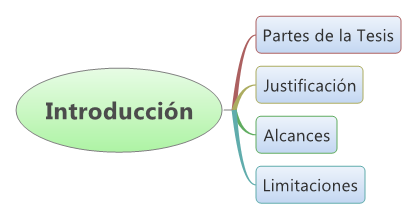
\includegraphics[scale=0.50]{./img/MapaMental/capitulo01.png}
		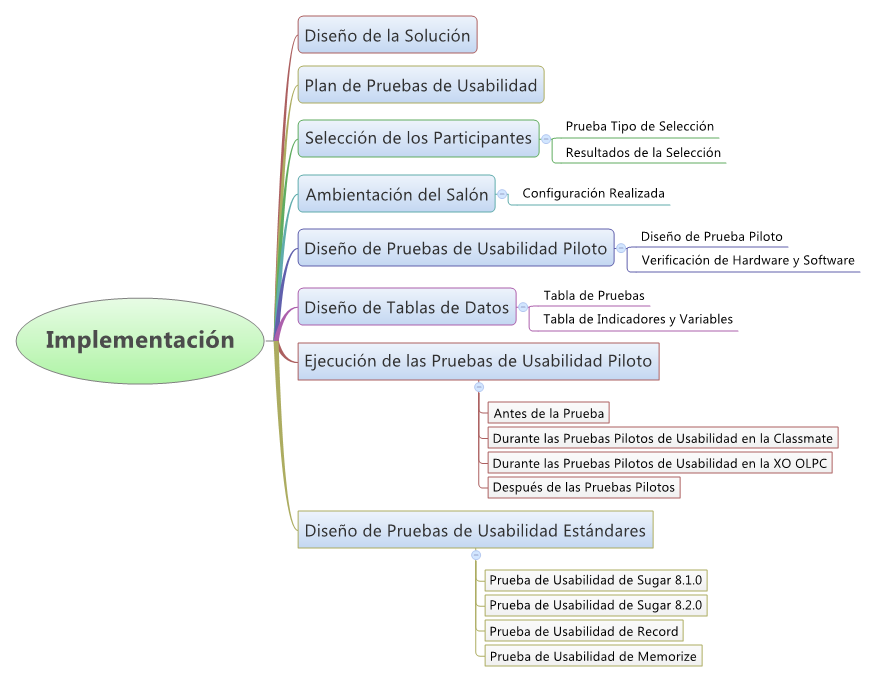
\includegraphics[scale=0.50]{./img/MapaMental/capitulo05.png}
	\caption{Mapa Mental del Cap�tulo de Implementaci�n}
	\label{Mapa Mental del Capitulo de Implementaci�n}
\end{figure}
 
% ----------------------------------------------
\section{Dise�o de la Soluci�n}
\label{section.Disenhiodelasolucion}




% ----------------------------------------------
\section{Plan de Pruebas de Usabilidad}
\label{section.PlandePruebasdeUsabilidad}

A continuaci�n se detalla el Plan de Pruebas de Usabilidad:


\textbf{1. Objetivos}: Realizar pruebas de usabilidad del software Sugar, escritorio de las laptops XO-1 de la OLPC. El objetivo del presente Plan de Pruebas es parte del Objetivo Superior de la Tesis en curso.\footnote{Secci�n \ref{subsection.Objetivo.Superior}}.

\textbf{2. Preguntas de investigaci�n}\footnote{Preguntas que se responder�n en las conclusiones.}:

\textbf{ - }�La ni�a o el ni�o usa la interf�z adecuadamente?.

\textbf{ - }�La ni�a o el ni�o usa con facilidad la OLPC XO?.

\textbf{ - }�La ni�a o el ni�o navegan adecuadamente en la interface gr�fica?.

\textbf{ - }�La ni�a o el ni�o ubican los iconos con facilidad?.

\textbf{ - }�La disposici�n de los objetos en una actividad facilitan el realizar la tarea a la ni�a o ek ni�o?

\textbf{ - }�Existe diferencia en usabilidad entre usar Sugar 8.1.0 y 8.2.0?

\textbf{ - }�Existe alguna relaci�n en realizar una tarea repetitiva en una Actividad Determinada y que en otra?

\textbf{ - }�La disposici�n de marcos es la m�s adecuada?

\textbf{ - }�El tama�o de los objetos es buena para la vista?	

\textbf{ - }�La muestra es la necesaria para la evaluar la usabilidad de este producto de Software?	

\textbf{3. Metodolog�a}: El uso de metodolog�as en las pruebas, ser� la siguiente, procurando ser estrictos en la recolecci�n de datos, el contexto de la evaluaci�n y las limitaciones de tiempo y recursos:	

\textbf{- Acuerdos con el Docente y Alumnos}: Antes de la realizaci�n de la prueba, se debe tener bajo acuerdo la participaci�n de la profesora del aula como de los alumnos.

\textbf{- Prueba de Selecci�n}: Se debe realizar una prueba de selecci�n para escoger a los alumnos con perfil necesario para las pruebas.

\textbf{- Piloto de Pruebas de Usabilidad}: Se deber� tomar una prueba piloto una ni�a y un ni�o, verificando el plan de Pruebas y las correcciones necesarias para las tareas a efectuar, mejora del ambiente de pruebas de usabilidad y est�ndares del estudio.

\textbf{- Compensaci�n}: No se realizar� pago alguno a los ni�os, se debe tener un acuerdo con la profesora para proporcionar materiales educativos en beneficio de los ni�os.

\textbf{- Ambientaci�n}: Antes de la prueba deber� ambientar el aula de clase donde se realizar�.

\textbf{- Material de Contingencia}: Durante la prueba	se debe tener el equipo de respaldo en caso de aver�a o fallo del equipo en prueba.

\textbf{- Distracciones}: Se debe evitar en lo posible tener la presencia de mas de un ni�o durante la prueba si esta no es con el uso de aplicaciones distribuidas.

\textbf{- Asistentes}: En caso de realizar mas de una prueba en un d�a se deber� tener un asistente para verificar el regreso del ni�o a su aula de clase y solicitar el permiso a la profesora para contar con el alumno oportuno y llevarlo al ambiente de pruebas.

\textbf{- Anulaci�n de Pruebas}: Si una prueba tiene muchos errores por nerviosismo del ni�o, por falta de inter�s, defectos en los instrumentos de grabaci�n. Deber� ser descartada y repetirse.


\textbf{4. Sesiones}: Las evaluaciones de usabilidad se llevar�n a 6 cada mes. Tratando de evitar la prolongaci�n a dos semanas entre prueba y prueba. Esta demora para realizar las pruebas de usabilidad es debido a que no se pod�a interrumpir de facto las clases del sal�n evaluar simultaneamente a un n�mero X de estudiantes y cada evaluaci�n debe realizarse en un sal�n de clases por lo tanto se debe acondicionar el ambiente para esto. Lo mas propicio era evaluar a uno o dos durante la semana el periodo de Junio a diciembre.

\textbf{5. Riesgos}: Se contemplan los siguientes riesgos:	

\textbf{ - }Permiso no concedido luego de tr�mites para realizar las pruebas en el colegio.

\textbf{ - }Falta de equipo, no entrega de la classmate, xo a tiempo.

\textbf{ - }Robo, p�rdida o da�o de equipos.

\textbf{ - }Reducci�n del presupuesto para llevar a cabo la investigaci�n.

\textbf{6. Acuerdos de Antes de la Pruebas}: Previo a la realizaci�n de las pruebas de usabilidad. Se firm� un compromiso con las profesora del aula: Sonia Fern�ndez Laz�n\footnote{Ver Anexo 1 Carta de Autorizaci�n.}.

\textbf{7. Introducci�n a la sesi�n}: Para el uso de las OLPC XO se tendr� una sesi�n de descripci�n previa a la prueba de usabilidad, adem�s se explicar� las tareas de la prueba de usabilidad enumerando las tareas y permitiendo al ni�o a realizar las preguntas.

\textbf{8. Rol del moderador}: El moderador es el tesista conjuntamente con una profesional de educaci�n o factores humanos que apoyar�n en la realizaci�n de la prueba.

\textbf{9. Configuraci�n del ambiente}: El Ambiente deber� estar limpio y aseado, evitar la corrientes de aire, ruido, exceso de luz solar y objetos que puedan desviar la atenci�n del ni�o durante la prueba.

\textbf{10. Especificaci�n de Tareas}: La especificaci�n de cada tarea ser� realizada por el moderador al momento de la sesi�n de pruebas. Se debe tener encuenta que en el Cap�tulo \ref{Diseno.de.la.Investigacion} se asocia el n�mero de tareas a una variable independiente.

\textbf{11. Prueba piloto}: La prueba usabilidad piloto deber� realizar lo mas antes teniendo los equipos de la classmate o olpc xo en el poder del moderador. 

\textbf{12. Pruebas est�ndar}: Las pruebas est�ndar deber�n de realizarse luego de tener la prueba de usabilida refinada de acuerdo a las observaciones recogidas de las pruebas de usabilidad piloto.

\textbf{13. Medidas}: Las medidas o m�tricas estas definidad en las Tablas \ref{TabladeDatosdePruebasdeUsabilidad}, \ref{VariablesIndependientesyDependiente} y 	\ref{TabladeIndicadores}.

\textbf{14. Informe de contenidos}: Los resultados de las pruebas de usabilidad se detallar�n en el Cap�tulo \ref{chapter.Analisis.de.Resultados}. Se deber� tener encuenta las estad�sticas y contrastes definidas en la Secci�n \ref{subsection.Contrastedehipotesis}. 

\textbf{15. Recomendaciones}: Las recomendaciones deber�n que englobar todo lo detallado para el estudio cuestiones fundamentales como la concepci�n de las interfaces gr�ficas.


Este Plan se orienta �nicamente a especificar la labor de los interesados y el procedimiento de las pruebas. No se dedundar� en datos te�ricos o metodolog�as ya explicadas. 

% ----------------------------------------------
\section{Selecci�n de los Participantes}
\label{section.SelecciondelosParticipantes}

Para el dise�o de la prueba de selecci�n se necesit� obligatoriamente el seguimiento y revisi�n de un profesor de primaria en computaci�n para ni�os. Se cont� con la asesor�a de la licenciada Elizabeth Benites Rojas\footnote{email: Elizabeth Benites Rojas elizabethbr(at)gmail(dot)com.}, Ketty Keynes Valdez\footnote{email: Ketty Keynes Valdez kettyenes(at)hotmail(dot)com.}, Natividad Gonzales Cordova\footnote{email: Natividad Gonzales Cordova solbezi(at)gmail(dot)com.}. Se toma como ejemplo algunos trabajo anteriores como de Janet \cite{02JanPanStuJoh2008} y \cite{Janet} sobre todo el uso de las pruebas de selecci�n favicon o las caras felices para que el ni�o escoja su valoraci�n.

\subsection{Prueba Tipo de Selecci�n}
\label{subsection.PruebaTipodeSelecci�n}



\subsection{Resultados de la Selecci�n}
\label{subsection.ResultadosdelaSeleccion}

\section{Ambientaci�n del Sal�n}
\label{section.AmbientaciondelSalon}




Sobre la lista de equipos y detalles se pude tener referencia en la Tabla \ref{MaterialesdelasPruebasdeUsabilidad} sobre Materiales y Equipos. 

\subsection{Configuraci�n Realizada}
\label{subsection.ConfiguracionRealizada}


% ----------------------------------------------
\section{Dise�o de Pruebas de Usabilidad Piloto}
\label{section.DisenhiodePruebasdeUsabilidadPiloto}


\subsection{Dise�o de Prueba Piloto} 
\label{subsection.DisenhiodePruebaPiloto}

\section{Dise�o de Tablas de Datos}
\label{section.DisenhiodeTablasdeDatos}


\subsection{Tabla de Pruebas}
\label{subsection.TabladePruebas}


\begin{table}[ht]
\scriptsize
	\centering
		\begin{tabular}{|m{3cm}|m{3cm}|}
		\hline			
\textbf{Variable} & \textbf{Descripci�n} \\\hline
\textbf{X1} &  \\\hline
\textbf{X2} &  \\\hline
\textbf{X3} &  \\\hline
\textbf{X4} &  \\\hline
\textbf{Y1} &  \\\hline
		\end{tabular}
	\caption{Variables Independientes y Dependiente}
	\label{VariablesIndependientesyDependiente}
\end{table}

La descripci�n de cada varaible se encuentra en la Secci�n \ref{subsection.Variablesindependientes}.
Los indicadores se extraer se detallaron en la Secci�n \ref{subsection.Indicadores}. Se colocar�n la siguiente tabla:

\begin{center}
\scriptsize
\begin{longtable}{|m{2.5cm}|m{1.35cm}|m{1.35cm}|m{1.35cm}|m{1.35cm}|m{1.5cm}|m{1.35cm}|m{1cm}|}
  \hline
\textbf{Indicador} & \textbf{Noa01X3} & \textbf{Noa02X3} & \textbf{Noa03X3} & \textbf{Noa04X3} & \textbf{Noa05X3} & \textbf{Noa06X3} & \\\hline 
\endfirsthead
  \hline
\textbf{Indicador} & \textbf{Noa01X3} & \textbf{Noa02X3} & \textbf{Noa03X3} & \textbf{Noa04X3} & \textbf{Noa05X3} & \textbf{Noa06X3} & \\\hline 
\endhead
\hline
	\caption{Tabla de Indicadores}
	\label{TabladeIndicadores}
\endlastfoot
\hline
\multicolumn{8}{|m{10.5cm}|}{Tabla de Indicadores}\\
\hline
\endfoot
%\footnotetext{Tabla de Indicadores}
\textbf{InPX2X4} & & & & & & & \\\hline
\textbf{InPX2X3X4} & & & & & & & \\\hline
\textbf{InPX1X4} & & & & & & & \\\hline
\textbf{InPX1PTTX4} & & & & & & & \\\hline
\textbf{InPX1PTTX3X4} & & & & & & & \\\hline
\textbf{InPPE} & & & & & & & \\\hline
\textbf{InNoComX4} & & & & & & & \\\hline	
\textbf{InRECX4} & & & & & & & \\\hline
\end{longtable}
\end{center}

\textbf{Nota:}
La descripci�n de cada indicador y su f�rmula se encuentra en la Secci�n \ref{subsection.Indicadores}.

\subsection{Tabla de Errores y Su Tratamiento}
\label{subsection.TabladeErroresySuTratamiento}


\begin{table}[ht]
\scriptsize
    \centering
%            \begin{tabular}{|m{1.2cm}|m{1cm}|m{1cm}|m{1cm}|m{1cm}|m{1cm}|m{1cm}|m{1cm}|m{1cm}|m{1cm}|m{1cm}|m{1cm}|}
\begin{tabular}{|m{1.2cm}|m{0.7cm}|m{0.7cm}|m{0.7cm}|m{0.7cm}|m{0.7cm}|m{0.7cm}|m{0.7cm}|m{0.7cm}|m{0.7cm}|m{0.7cm}|m{0.7cm}|}
                    \hline
                    &\textbf{Y1}&\textbf{Y2}&\textbf{Y3}&\textbf{Y4}&\textbf{Y5}&\textbf{Y6}&\textbf{Y7}&\textbf{Y8}&\textbf{Y9}&\textbf{Y10}& \\\hline
                    \textbf{Noa01X3} &&&&&&&&&&&\\\hline
                    \textbf{Noa02X3} &&&&&&&&&&&\\\hline
                    \textbf{Noa03X3} &&&&&&&&&&&\\\hline
                    \textbf{Noa04X3} &&&&&&&&&&&\\\hline
                    \textbf{Noa05X3} &&&&&&&&&&&\\\hline
                    \textbf{Noa06X3} &&&&&&&&&&&\\\hline
                    \textbf{Promedio}&&&&&&&&&&&\\\hline
                  \end{tabular}
             \caption{Tabla de La Probabilidad de Errores de Usabilidad}
     \label{TabladeLaProbabilidaddeErroresdeUsabilidad}
\end{table}



% ----------------------------------------------
\section{Ejecuci�n de las Pruebas de Usabilidad Piloto}
\label{section.EjecuciondelasPruebasdeUsabilidadPiloto}

Las pruebas piloto de usabilidad se desarrollaron en junio y julio del 2008, las visitas demoraron porque reci�n se obtuvo los equipos de laptops (la Classmate fue prestada por un mes, Figura \ref{Recibo del Pr�stamo de la ClassMate} del Anexo 3. Las OLPC XO-1 fueron donadas por el proyecto OLPC como contribuyente, Figura \ref{Recibo de Donaci�n de las OLPC} del Anexo 2.) y se estaba acondicionando su uso para lo ni�os como se se�alo en la Secci�n \ref{VerificaciondeHardwareySoftware}.

\begin{table}[ht]
\footnotesize
    \centering
            \begin{tabular}{|m{3.2cm}|m{1.2cm}|m{1.8cm}|m{1.4cm}|m{2cm}|}
             \hline
            Video & \textbf{Tiempo} & \textbf{Segundos} & \textbf{Tama�o} & \textbf{Resoluci�n}\\\hline
            naSugarOLPC.avi& 04:01& 241 &25MB&720x480\\\hline
            naSugarClassmate.avi& 10:09& 609& 65MB&720x480\\\hline
            noSugarOLPC.avi& 06:27& 387 &41MB&720x480\\\hline
            noSugarClassmate.avi &10:01 &601& 64MB&720x480\\\hline
            \end{tabular}
    \caption{Tiempos de las Pruebas Piloto}
\label{Tiempos de las Pruebas Piloto}
\end{table}


\subsection{Antes de la Prueba}
\label{subsection.AntesdelaPrueba}

Las pruebas de usabilidad se realizaron los d�as jueves a las 11:00 am. Es una hora luego del recreo de los ni�os. Antes de realizar la prueba se acondicion� el ambiente limpi�ndolo y ordenando el moviliario para colocar los equipos de la laptop, c�mara filmadora y papel�grafos. Se tuvo la participaci�n de la profesora de clases para la fase de Entrada.

\subsection{Durante las Pruebas Pilotos de Usabilidad en la Classmate}
\label{subsection.DurantelaPruebaClassmate}

Se llev� a cabo las pruebas pilotos de usabilidad usando las tareas presentadas en la secci�n \ref{subsection.DisenhiodePruebaPiloto}. Para ambos ni�os en d�as distintos. Se escogi� la prueba del ni�o por tener la mayor cantidad de problemas u obst�culos a la prueba realizada por la ni�a.
El tiempo promedio de ambos desarrollos del test fue de 9 minutos teniendo un planeamiento de 10 minutos al inicio.


\subsection{Durante las Pruebas Pilotos de Usabilidad en la XO OLPC}
\label{subsection.DurantelaPruebaXO}

Para realizar las pruebas de usabilidad en las XO de la OLPC se debi� proceder con lo descrito en la secci�n \ref{VerificaciondeHardwareySoftware}. Se cargo dos bater�as para las pruebas por cada d�a por si se consum�a mas de lo debido. En la Figura \ref{PruebaPilotodeUsabilidadenlaOLPC} se notan ambas pruebas. 

\section{Dise�o de Pruebas de Usabilidad Est�ndares}
\label{section.DisenhiodePruebasdeUsabilidadEstandares}

Se coloca a continuaci�n las tareas de las pruebas de usabilidad formales realizadas durante la investigaci�n. Se realiz� las pruebas de usabilidad a 6 ni�os y 6 ni�as durante el periodo del agosto a diciembre del 2008.
Cada prueba de usabilidad  tiene un desarrollo por un tiempo adecuado a su prueba y adem�s los datos est�n volcados en los anexos \ref{chapter.anexos}.

\subsection{Prueba de Usabilidad de Sugar 8.1.0}
\label{subsection.PruebadeUsabilidaddeSugar8.1.0}

	\textbf{- T1X2}: Ubicar el Cursor en la Pantalla.
	
	\textbf{- T2X2}: Ubicar el icono de Vecindario.
	
	\textbf{- T3X2}: Hacer click en el icono de vecindario.
	
	\textbf{- T4X2}: Ubicar el icono de Escuela.
	
	\textbf{- T5X2}: Hacer click en el icono de Escuela.
	
	\textbf{- T6X2}: Ubicar el icono de Actividad.
	
	\textbf{- T7X2}: Hacer click en el icono de Actividad.
	
	\textbf{- T8X2}: Ubicar el icono de Casa.
	
	\textbf{- T9X2}: Hacer click en el icono de Casa.
	
	\textbf{- T10X2}: Ubicar el cursor en el centro de la pantalla.
	
	\textbf{- T11X2}: Ubicar la letra "A" de la palabra Acerca.
	
	\textbf{- T12X2}: Hacer click en la palabra Acerca.
	
	\textbf{- T13X2}: En el cuadro Hacer click en la Palabra Aceptar.	


\subsection{Prueba de Usabilidad de Sugar 8.2.0}
\label{subsection.PruebadeUsabilidaddeSugar8.2.0}

  \textbf{- T1X2}: Ubicar el Cursor en la Pantalla.
	
	\textbf{- T2X2}: Ubicar el icono de Vecindario.
	
	\textbf{- T3X2}: Hacer click en el icono de vecindario.
	
	\textbf{- T4X2}: Ubicar el icono de Escuela.
	
	\textbf{- T5X2}: Hacer click en el icono de Escuela.
	
	\textbf{- T6X2}: Ubicar el icono de Actividad.
	
	\textbf{- T7X2}: Hacer click en el icono de Actividad.
	
	\textbf{- T8X2}: Ubicar el icono de Casa.
	
	\textbf{- T9X2}: Hacer click en el icono de Casa.
	
	\textbf{- T10X2}: Ubicar el Icono Organizar esperar que se despliegue.
	
	\textbf{- T11X2}: Hacer Click en uno de los iconos parecidos.
	
	\textbf{- T12X2}: Ubicar el centro de la pantalla esperar el despliegue del menu
	
	\textbf{- T13X2}: Hacer click en panel de Control.
	
	\textbf{- T14X2}: Ubicar el icono de Salir.
	
	\textbf{- T15X2}: Hacer click sobre el icono de Salir.
	


\subsection{Prueba de Usabilidad de Record}
\label{subsection.PruebadeUsabilidaddeRecord}

	
	\textbf{- T1X2}: Ubicar el cursor en la pantalla.
	
	\textbf{- T2X2}: Ubicar el icono de Record.
	
	\textbf{- T3X2}: Hacer click en el icono Record.
	
	\textbf{- T4X2}: Ubicar el icono de tomar Foto en Record.
	
	\textbf{- T5X2}: Darle click en el icono de Tomar Foto.
	
	\textbf{- T6X2}: Ubicar la foto tomada.
	
	\textbf{- T7X2}: Darle click en la foto tomada.
	
	\textbf{- T8X2}: Pasar el cursor sobre la foto tomada hacer click en el icono de ampliaci�n.
	
	\textbf{- T9X2}: Pasar el cursor sobre el video para ir a modo normal.
	
	\textbf{- T10X2}: Ubicar la pesta�a Video.
	
	\textbf{- T11X2}: Hacer click sobre la pesta�a de video.
	
	\textbf{- T12X2}: Ubicar el icono de grabar video.
	
	\textbf{- T13X2}: Darle click en el icono de grabar video.
	
	\textbf{- T14X2}: Darle click en el video tomado.
	
	\textbf{- T15X2}: Pasar el cursor sobre la foto tomada hacer click en el icono de ampliaci�n.
	
	\textbf{- T16X2}: Pasar el cursor sobre el video para ir a modo normal.
	
	\textbf{- T17X2}: Ubicar la pesta�a Actividad.
	
	\textbf{- T18X2}: Hacer click en la pesta�a Actividad.
	
	\textbf{- T19X2}: Dirigirse al icono de cerrar.
	
	\textbf{- T20X2}: Hacer click sobre la pesta�a de salir.		



\subsection{Prueba de Usabilidad de Memorize}
\label{subsection.PruebadeUsabilidaddeMemorize}

	\textbf{- T1X2}: Ubicar el Cursor en la Pantalla.
	
	\textbf{- T2X2}: Ubicar el icono de Memorize.
	
	\textbf{- T3X2}: Hacer click en el icono Memorize.
	
	\textbf{- T4X2}: Ubicar la pesta�a Actividad.
	
	\textbf{- T5X2}: Hacer click en las casillas 1 de la parte superior.
	
	\textbf{- T6X2}: Hacer Click en las casillas 2 de la parte inferior.
	
	\textbf{- T7X2}: Completar el juego.
	
	\textbf{- T8X2}: Hacer click en la pesta�a Actividad.
	
	\textbf{- T9X2}: Dirigirse al icono de cerrar.

	\textbf{- T10X2}: Hacer click sobre la pesta�a de salir.


 %8. Modelo de Soluci�n
%\chapter{AN�LISIS DE RESULTADOS}
%\vspace*{8cm}
\chapter{An�lisis de Resultados}
\label{chapter.Analisis.de.Resultados}
% ----------------------------------------------

\begin{figure}[ht]
	\centering
		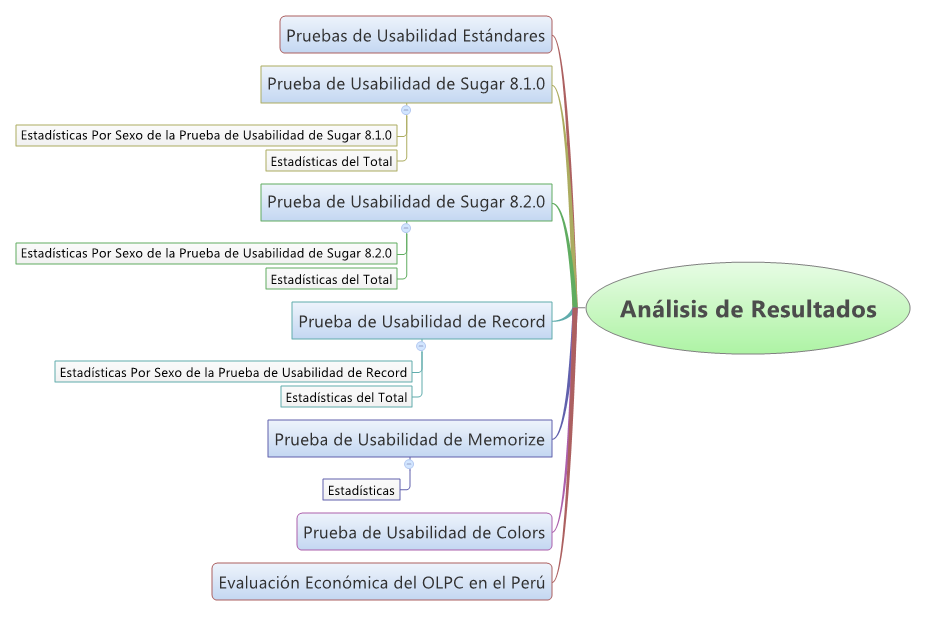
\includegraphics[scale=0.50]{./img/MapaMental/capitulo061.png}
	\caption{Mapa Mental del Cap�tulo de An�lisis de Resultados}
	\label{Mapa Mental del Capitulo de An�lisis de Resultados}
\end{figure}


% ----------------------------------------------
\section{Desarrollo de Pruebas de Usabilidad Est�ndares}
\label{section.DesarrollodePruebasdeUsabilidadEstandares}

El total de las pruebas de usabilidad realizadas de forma satisfactoria\footnote{No se cuentas las pruebas fallidas o mal ejecutadas por problemas de los equipos o por demasiado nerviosismo del usuario por ejemplo el exceso de sudoraci�n en las manos luego de una actividad de educaci�n f�sica.} se muestra en la Tabla \ref{CuadroDePruebasDeUsabilidad}. 

\begin{table}[ht]
\footnotesize
	\centering
	\begin{tabular}{|m{7cm}|m{1.2cm}|m{1.2cm}|}
		\hline	
 & \textbf{Ni�os} & \textbf{Ni�as}\\\hline
\multicolumn{3}{|m{9.4cm}|}{OLPC Sugar Build 703 Rel. 8.1.0} \\\hline
Test de Usabilidad de Sugar Desktop	& 6	& 6\\\hline
Test de Usabilidad de Grabar & 6 & 6\\\hline
Test de Usabilidad de Memoria & 3 & 3\\\hline
Test de Usabilidad de Pintar & 1 & 1\\\hline
\multicolumn{3}{|m{9.4cm}|}{OLPC Sugar Build 656 Rel. 7.2.0} \\\hline
Test Piloto de Usabilidad de Turtle Art &	1 & 1\\\hline
\multicolumn{3}{|m{9.4cm}|}{ClassMate Ubuntu} \\\hline
Test Piloto de Usabilidad de Turtle Art &	1 &	1\\\hline
\multicolumn{3}{|m{9.4cm}|}{OLPC Sugar Build 767 Rel 8.2.0} \\\hline
Test de Usabilidad de Sugar Desktop	& 6 &	6\\\hline
Totales	& 24 &	24\\\hline
		\end{tabular}
	\caption{Cuadro de Pruebas de Usabilidad}
	\label{CuadroDePruebasDeUsabilidad}
\end{table}

El an�lisis de las pruebas de usabilidad se realizar�n por cada prueba.
Las pruebas de usabilidad fueron registradas por medio de filmaciones digitales. Cada uno de estos videos fue procesado en las Tablas \ref{TiempoparaSugar081}, \ref{TiempoparaSugar082}, \ref{TiempoparaRecord}, \ref{TiempoparaMemorize} se tiene la descripcion de cada prueba de usabilidad el tama�o, el tipo de compresi�n usado fue wmv1\footnote{WMV no se construye s�lo con tecnolog�a interna de Microsoft. Desde la versi�n 7 (WMV1), Microsoft ha utilizado su propia versi�n no estandarizada de MPEG-4. El v�deo a menudo se combina con sonido en formato Windows Media Audio. Extraido de http://es.wikipedia.org/wiki/Windows\_Media\_Video 12/10/2009} se  intent� usar el formato ogv\footnote{Ogg encapsula datos comprimidos (e incluso sin comprimir) y permite la interpolaci�n de los datos de audio y de v�deo dentro de un solo formato conveniente. Extraido de http://es.wikipedia.org/wiki/Ogg 12/10/2009. P�gina del Proyecto http://www.xiph.org/ogg/ 12/10/2009.} pero se tuvo muchas p�rdidas en los cuadros. Cada uno de las pruebas se muestran en el Anexo \ref{section.anexo.10} en un despliegue de 12 cuadros.
% ----------------------------------------------//
\section{Desarrollo de Prueba de Usabilidad de Sugar 8.1.0}
\label{section.Desarrollo de Prueba de Usabilidad de Sugar 8.1.0}

\section{Desarrollo de Prueba de Usabilidad de Record}
\label{section.DesarrollodePruebasdeUsabilidadEstandares}

\subsection{Descripci�n del Modelo y Procedimiento}
\label{subsection.Descripci�n.del.Modelo}

 %9. Medici�n de la Usabilidad de la OLPC % Instrumentos de Medici�n
%\chapter{CONCLUSIONES}
%\chapter{CONCLUSIONES Y RECOMENDACIONES}
%\vspace*{8cm}
\chapter{Conclusiones y Recomendaciones}
\label{chapter.conclusiones}

% ----------------------------------------------

\begin{figure}[ht]
	\centering
		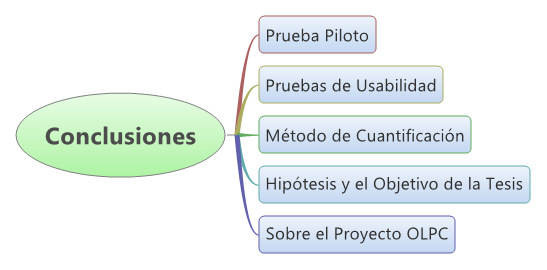
\includegraphics[scale=0.60]{./img/MapaMental/conclusiones.png}
	\caption{Mapa Mental del Cap�tulo de Conclusiones}
	\label{Mapa Mental del Capitulo de Conclusiones}
\end{figure}



\section{Conclusiones}
\label{section.Conclusiones}

\section{Recomendaciones}
\label{section.Recomendaciones}
 %11. Conclusiones
\glosario
\newpage
\bibliography{references}
\newpage
%\chapter{Anexos}
%\vspace*{8cm}
%\vskip3cm 
%\chapter*{\vskip1cm Anexos}
\chapter*{Anexos}
\addcontentsline{toc}{chapter}{Anexos}
%\chapter{ANEXOS}
\label{chapter.anexos}

% ----------------------------------------------
%\newpage
\section*{Anexo 1: Carta de Autorizaci�n}
\addcontentsline{toc}{section}{Anexo 1: Carta de Autorizaci�n}
\label{section.anexo.1}
Carta de la profesora aceptando la realizaci�n de las pruebas de usabilidad a los alumnos de colegio.

\begin{figure}[ht]
	\centering
		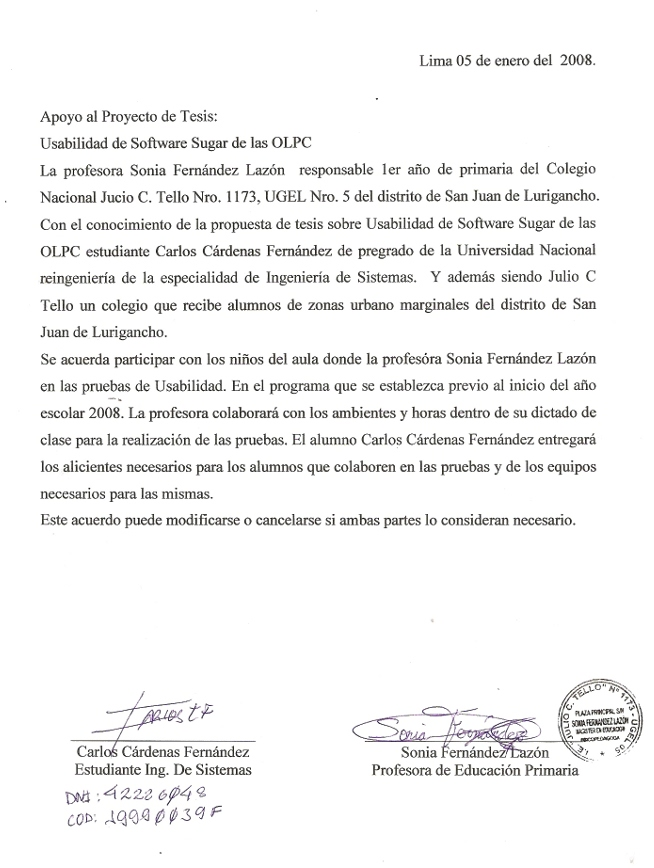
\includegraphics[scale=0.38]{./img/escanear0006.jpg}
	\caption{Carta de Autorizaci�n de la Profesora}
	\label{Carta de Autorizaci�n de la Profesora}
\end{figure}

% ----------------------------------------------
\newpage
\section*{Anexo 2: Recibo de Donaci�n de las OLPC}
\addcontentsline{toc}{section}{Anexo 2: Recibo de Donaci�n de las OLPC}
\label{section.anexo.2}
Recibo de Donaci�n de las OLPC.
\begin{figure}[ht]
	\centering
		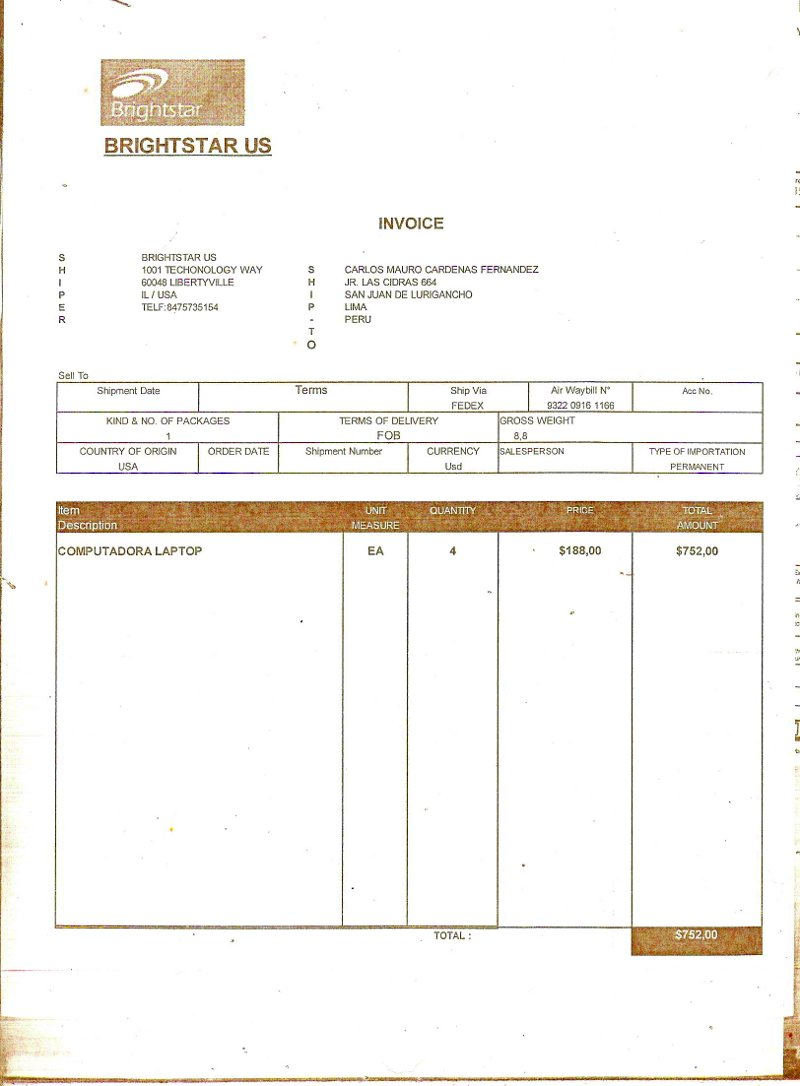
\includegraphics[scale=0.40]{./img/escanear0003.jpg}
	\caption{Recibo de Donaci�n de las OLPC}
	\label{Recibo de Donaci�n de las OLPC}
\end{figure}

% ----------------------------------------------
\newpage
\section*{Anexo 3: Recibo del Pr�stamo de la ClassMate.}
\addcontentsline{toc}{section}{Anexo 3: Recibo del Pr�stamo de la ClassMate.}
\label{section.anexo.3}
Recibo del Pr�stamo de la ClassMate.
\begin{figure}[ht]
	\centering
		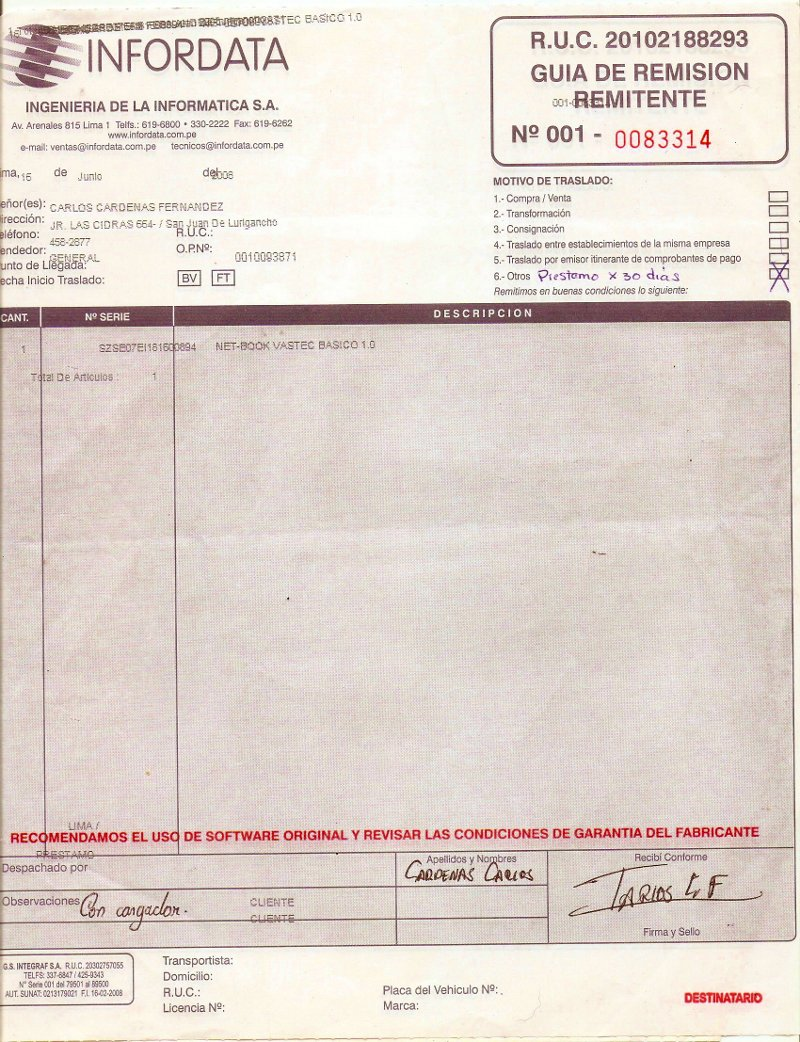
\includegraphics[scale=0.45]{./img/escanear0002.jpg}
	\caption{Recibo del Pr�stamo de la ClassMate}
	\label{Recibo del Pr�stamo de la ClassMate}
\end{figure}


 %13. Anexos


\newpage
\univita
\unicopyright


\end{document}
